\documentclass[onecolumn]{IEEEconf}
\usepackage{enumitem}
\usepackage[usenames, dvipsnames]{color}
\usepackage{graphicx}
\usepackage{subcaption}
\usepackage{tabularx,calc}
\usepackage{url}
\usepackage{amsmath}
\usepackage{comment}
\usepackage{commath}
\usepackage[utf8]{inputenc}
\usepackage{xcolor}
\usepackage{mdframed}
\usepackage[normalem]{ulem}
%\usepackage{algorithm}
\usepackage[linesnumbered,ruled,vlined]{algorithm2e}
\usepackage{multirow}
\newcommand{\red}[1]{{\textcolor{red}{#1}}}
\usepackage{ragged2e}
\usepackage{capt-of}
\usepackage{amssymb}% http://ctan.org/pkg/amssymb
\usepackage{pifont}% http://ctan.org/pkg/pifont
\newcommand{\cmark}{\ding{51}}%
\newcommand{\xmark}{\ding{55}}%
\renewcommand{\figurename}{Fig.}
\renewcommand*{\thetable}{\Roman{table}}
\usepackage[utf8]{inputenc}
\usepackage{kotex}

\newcommand{\old}[1]{\textcolor{red}{\sout{#1}}}
\newcommand{\new}[1]{\textcolor{blue}{#1}} 
\newcommand\mc[1]{\multicolumn{1}{c}{#1}} % handy shortcut macro

\SetKwInput{KwInput}{Input}                % Set the Input
\SetKwInput{KwOutput}{Output}              % set the Output
\let\oldnl\nl% Store \nl in \oldnl
\newcommand{\nonl}{\renewcommand{\nl}{\let\nl\oldnl}}
\newenvironment{algotabularx}
 {\tabularx{\linewidth-\inoutsize-\widthof{~~~}-4\tabcolsep-\rightskip}[t]}

\title{Response to the Reviewers\\VT-2019-03792}
\begin{document}
\maketitle

\setlength{\parindent}{0cm}
\textbf{\large Editors Comments:}\\
The reviewers and the editor recognize scientific interest in the manuscript, particularly the exploitation of optimization methods to minimize energy consumption of UAVs. However, the manuscript, in its present form, suffers from several technical and presentation weaknesses, which needs to be addressed. 
Some of the concerns raised by the reviewers are:~\\
\textcolor{red}{김재민 교수님이나, 백돈규 교수님께 받은 RR에서는 에디터를 위한 답변은 달리 존재 하지 않았었는데 에디터에게 쓰는 답변은 초본 검토 후에 작성하는게 좋을 것 같습니다. 대신 답변을 위한 내용들을 개괄식으로 작성하겠습니다.}
\begin{description}
    \item \textbf
	{
	C1: The literature review lacks discussion of recent papers, particularly the ones published in the last 3-4 years; 
	}
	\item \textit
	{
	R1: 리뷰어 3은 현재 트랜드에 맞는 새로운 논문들을 레퍼런스에 추가하길 바라며, 리뷰어 4는 introduction 과 relate works를 조금 더 축약해주길 원합니다.\\
	리뷰어 3이 추천해준 논문과 현재 트랜드에 적합한 강화 학습을 이용한 논문을 레퍼런스와 related work에 추가하였고, Section 1,2 를 다시 검토해 내용을 축약하였습니다. 
	}
	~\\
	~\\
	\item \textbf
	{
	C2: The presentation of the optimization-based flight plan methods needs more technical detail and insights. For example, the mathematical formulation of the optimization problem is unclear, the sensing requirements need to be more precisely defined (in particular the measurement of  wind velocity) and the discussion of the real-time applicability of the method is vague.
	}
	\item \textit
	{
	R2: 우리는 Section 6에 새롭게 추가한 subsecion 6-A 에서 우리의 드론의 임무 최적화 과정의 문제를 포뮬레이션 하였으며, 이어지는 Subsection 6-C, 6-D 에 알고리즘들을 통하여 문제를 해결하는 방법을 제시합니다.~\\
	파워 모델 형성을 위하여 사용한 wind sensor에 관한 내용은 Subsection IV-D에 추가적으로 작성하였고, 저희가 현재 최적화를 진행하고 있는 환경이 온라임이 아님을 언급하며 대체제인 CFD를 Subsection 6-B 에 서술하였습니다.	}
    ~\\
    ~\\
	\item \textbf
	{
	C3: Validation of the method under more challenging conditions (e.g. time-varying wind velocity) is encouraged
	}
	\item \textit
	{
	R3: 이 역시 저희가 온라인이 아닌 오프라인 상황에서 최적화를 진행함을 Section 6 에서 언급 하였으며 대신 현실에서 사용할 수 있을 만큼의 최적화 결과를 얻기 위해 우리는 최적화 환경을 CFD를 이용하여 보강 하였음을 Subsection 6-B 에 서술하였습니다.
	}
	~\\
	~\\
	\item \textbf
	{
	C4: From a presentation perspective, the manuscript also requires an English proofread 
	}
	\item \textit
	{
	R4: 현재 김재민 교수님과 함께 다시 한번 논문을 체크 하고 있으며, 남은 기간 동안에도 꾸준히 수정하고 확인하겠습니다.
	}
	~\\
	~\\
\end{description}
    
\textbf{\large Reviewer 1:}\\
\begin{description}
    \item \textbf
	{
	C1: There are many grammar errors. You may want to double-check your sentences. For example,  Page 12 Line 15, "we demonstrate a example" should be "we demonstrate an example". This kind of mistake should be avoided. 
	}
	\item \textit
	{
	R1: We sincerely apologize for many grammar errors. We carefully double-checked whole the manuscript and fully revised sentences. We denoted changed sentences as red color. We appreciate your invaluable comments.
	}
	~\\
    ~\\
\end{description}

\textbf{\large Reviewer 2:}\\
It's a good paper, but I feel that it's missing an element of novelty or analytical rigor.  I think theres some more things that can be done to complete it.
As the UAS industry continues to expand and with the promise of drone delivery services just around the corner, I think there's an opportunity to be more forward looking to stand out.
\begin{description}
    \item \textbf
	{
	C1: Compare power consumption modeling techniques to demonstrate the value added by the DNN, ie, does the increased model accuracy have an appreciable difference on the performance of the path optimization. Is your model accuracy the best of all existing approaches? 
	}
	\item \textit
	{
	R1: We really appreciate your encouraging comment. Yes, our DNNs model has the most accurate power prediction compared with other models. We presented the results of comparing the DNNs model with the existing methodologies in the newly added Subsection V-C.
    %According to our result, the DNNs model is the highest accuracy compared with other models.
    However, predicting power consumption through neural networks is relatively slower than using numerical formulas, and the neural networks require a lot of effort to build the model through training: The DNNs model has a trade-off relationship between accuracy and speed.
    ~\\~\\
    On the other hand, the DNNs model clearly has an advantage in the accuracy, which is required when performing a large-scale search such as an optimal path planning rather than a real-time search that requires continuous fast power consumption prediction.
    We progressed offline planning according to the optimization scenario and problem formulation of Section~VI, and we proceeded with optimization through the graph search algorithm in the discretized simulation environment.
    In the discretized simulation environment, the amount of energy consumption calculated for each step of the environment becomes an essential factor in determining the path of the drone.
    Therefore, we use the highest accurate model (DNNs) to predict the power consumption in each step of the process for optimizing drone operations.
	}
	~\\
    ~\\
    \textcolor{red}{수정을 위해 라인 넘버는 우선 비워두겠습니다.}\\
	\textbf{We added new Subsection V-C in the manuscripts as follows (Page 7, Line ZZ.)}\\
    \begin{mdframed}[ linewidth=.75pt, userdefinedwidth=0.9\textwidth]
    \textbf{C. \textcolor{red}{Comparison of the power modeling methodologies}}~\\
    ~\\
    \textcolor{red}{Our proposed DNNs model consists of simple variables that represent simple drone movement and external forces. It does not require complex knowledge of the dynamics or control theory and has a high enough accuracy of about 90~\% compared with the actual flight data.}
    \textcolor{red}{We present prediction results of the proposed DNNs model, the model using momentum theory\,[5], the model using aerodynamics\,[3], and the data-driven model using the linear regression in Table\,III [10].
    As a result above, the DNNs model is the highest accuracy compared with other models.
    However, predicting power consumption through neural networks is relatively slower than using numerical formulas, and the neural networks require a lot of effort to build the model through training: The DNNs model has a trade-off relationship between accuracy and speed.
    Clearly, the DNNs model has an advantage in the accuracy, which is required when performing a large-scale search such as an optimal path planning rather than a real-time search that requires continuous fast power consumption prediction.
    Therefore, we use the highest accurate model (DNNs) to predict the power consumption in each step of the process for optimizing drone operations.
    We configure the power model of the drone so far, and we introduce the optimization of the minimum energy path of the drone using the power model configured in Section\,VI that follows.}
    ~\\
    \end{mdframed}
    ~\\
    \textbf{We also added new Table III. in the manuscripts as follows (Page 8.)}\\
    \begin{mdframed}[ linewidth=.75pt, userdefinedwidth=0.9\textwidth]
    \centering
    \textcolor{red}{
    \textbf{TABLE III Comparison of the result accuracy between power models}~\\
    %\resizebox{0.38\textwidth}{!}{%
    \begin{tabular}{|c|c|}
    \hline
    {Power modeling method} &  {Error rate (\%)} \\ \hline
    {Aerodynamics\,[3]}          & { 14.90}           \\ \hline
    {Data-driven\,[10]}           & { 13.73}           \\ \hline
    {Momentum theory + translocation term\,[5]}       & { 10.07}           \\ \hline
    {Deep neural networks}  & { 9.27}            \\ \hline
    \end{tabular}%
    %}
    }
    \end{mdframed} 
	~\\
	~\\
    \item \textbf
    {
	C2: Incorporate real-time power management adjustments - I think you could utilize the power consumption model in real-time to make adjustments to maintain optimal path planning in the event of changes in wind direction/speed. Or maybe consider multiple aircraft and some paths may not be feasible due to collision hazards.
	}
	\item \textit
	{
	R2: In the modeling process, we installed a wind sensor on the drone, collected the wind data in real-time, and included this data into a learning dataset to configure the power consumption because the wind affects a significant influence on the drone’s power consumption.
    Apart from the modeling, in the optimization process, the online planning involves several problems using wind data as a parameter.~\\~\\
    * First of all, the more parameters to consider in the optimization, the more complex the optimization problem becomes. The on-board computer of the drone is not suitable for handling huge computations in real-time.~\\~\\
    * Second, even if the drone receives the computation results that are solved externally, the drone must deliver wind information to the server for the calculation in real-time. It means the drone requires the additional cost for long-distance communications. Moreover, our goal of the research is to reduce the energy consumption of the drone without significant hardware improvements. The online planning method is not suitable for us.~\\~\\
    Therefore, we present the offline planning that transmits the optimal path derived by the base station that computes complex computation to the drone under the assumption that there is no sudden accident (e.g., bird strike). However, the offline planning also requires wind information at every grid cell of the simulation environment. In order to derive the optimal path for reality, the simulation environment must be as similar as possible to the actual conditions. We used the computational fluid dynamics (CFD) to interpret the wind flow and made it in the form of a discretized wind map to improve the offline simulation environment close to reality.~\\~\\
    We used the Dijkstra algorithm, a graph search algorithm, to solve the optimization problem by selecting an edge with the smallest energy consumption among edges connected to the same node. The derived path through edges of the graph is the optimal solution in the discretized environment.    This paper aims to find an optimal energy path for a single drone and a given environment. We do not address the collision issues that occur when multiple drones are in operation.
	~\\
    ~\\
    In the manuscript, we added a Subsection to clearly reveal our offline approach as follows:~\\
}
\textcolor{red}{
\textcolor{red}{\textit{A. The scenario of the drone optimization process.}}~\\~\\
In our scenario, the operator inputs information about a starting point and a destination to the main station to assign a task to the drone, as shown in Fig.\,8.
The station holds the power consumption model of the drone and wind maps about the operating environment, and the station derives the path between points entered from the operator.
% Offline 최적화임을 여기서 언급
Since the optimization is performed offline at the main station, it is impossible to modify the optimal path already drawn while the drone is running. Also, in this paper, we do not assume that the station considers the unexpected situations such as bird-strike or wind-sheer.
% 외부 바람을 고려하기 위해 전용 툴을 쓴다는 것을 여기서 언급함
However, we analyze the predictable external forces such as wind level and direction using the sophisticated analysis tool to take full advantage of the effects of external forces in creating the optimal path of the drone. 
After that, the drone receives the optimized path from the station and then runs to the destination along the path. We formulate the flight energy optimization problem of the drone as the following:}
\\
\\
\end{description}
~\\
~\\
~\\
\textbf{\large Reviewer 3:}\\
The paper is an interesting study, which focuses on a deep learning based method to develop a better power consumption model for multirotors.
This model is then used an optimization strategy for energy consumption minimization. It is indeed an important topic, since currently flight endurance is one of the important obstacle for the use of drones for various scientific, research and commercial purposes. The reviewer humbly suggests the authors to kindly consider following points for their study, and hopes that these will help the authors.
\begin{description}
    \item \textbf
	{
	C1: Literature review:
    Some relevant references are missing in the literature review. An example is the recent work by A.Mohiuddin et al[1]. where real time dynamic programming is used for a multi-criteria optimization to either save energy or time. This is appropriate for Table I. as well, since the latest study included in this table is from 2017. The authors are encouraged to look for new studies, that came after 2017 and add them to Table I.~\\~\\
    Mohiuddin, A.; Taha, T.; Zweiri, Y.; Gan, D. UAV Payload Transportation via RTDP Based Optimized Velocity Profiles. Energies 2019, 12, 3049~\\~\\
    Adding adequate but recent references, not only strengthen the paper, but also shows that the topic is of interest for the scientific community.
	}
	\item \textit
	{ 
	R1: We appreciate the reviewer for kind advice. We carefully check the recommended paper, and refer it in Section~II. We also contained an online planning paper of the drone using reinforcement learning to our references, which is appropriate for recent trends.
    By adding these two latest papers, we listed the literature reviews in Section II and have revised Table I, the result of our literature review, to the following.  
	}
    ~\\
    ~\\
	\textbf{We added references in the manuscripts as follows (Page 14.)}\\
    \begin{mdframed}[ linewidth=.75pt, userdefinedwidth=0.9\textwidth]
    \textcolor{red}{[4] Abdullah Mohiuddin, Tarek Taha, Yahya Zweiri, and Dongming Gan. Uav payload transportation via rtdp  based optimized velocity profiles. Energies, 12(16):3049, Aug 2019.} \\
    \textcolor{red}{[13] S. Shin, Y. Kang, and Y. Kim. Automatic drone navigation in realistic 3d landscapes using deep reinforcement learning. 
    In 2019 6th International Conference on Control, Decision and Information Technologies (CoDIT), pages 1072–1077, 2019.}
    \end{mdframed} 
	~\\
    \textbf{We modified Section~II in the manuscript as follows (Page 02, Line 87.)}\\
    \begin{mdframed}[ linewidth=.75pt, userdefinedwidth=0.9\textwidth]
    \textcolor{red}{A. Mohiuddin~et~al focus on the real-time optimization of the drone\,[4]. 
    The authors infer the optimal velocity of the drone to proceed to the next states based on the current state of the drone as an agent in the environment.
    They predict the power consumption of the drone through the dynamics-based power consumption model and optimal velocity inferred by the real-time dynamic programming.
    Reinforcement learning is one of the optimization solutions\,[13]
    They focus on solving the task problem of the drone in the partially observable Markov decision process. 
    They utilize Convolutional neural networks that use convolutional filters to detect edges of the picture taken by the drone and extract the characteristics of the image, and they predict the best action at each step in the discretized environment using Double deep Q networks.}
    \end{mdframed}
    ~\\
	~\\
    \textbf{We also modified TABLE~I. in the manuscript as follows (Page 3.)}
    %\begin{table*}[h]
    \begin{mdframed}
    \textbf{Table I.} Comparison of previous works for \textcolor{red}{the} drone optimization.
    \centering
    \label{Table: survay_result}
    \begin{tabular}{|c|c|c|c|c|c|}
    \hline
    \small Reference & \small Wind & \small Payload & \small Surface area & \small Optimization method & \small Goal \\ \hline
    %TVLSI 2019 & \cmark & \cmark & \cmark & Dijkstra algorithm & \multicolumn{1}{l|}{Minimum energy} \\ \hline
    \small ICARSC 2015~[10] & %\xmark 
    & %\xmark 
    & %\xmark 
    & \small Back-and-forth algorithm & \small Minimum energy \\ \hline
    \small IROS 2016~[6] & \cmark & %\xmark 
    & %\xmark 
    & \small Model predictive control & \small Minimum energy \\ \hline
    \small ICRA 2016~[8]  & %\xmark 
    & \cmark & %\xmark 
    & \small SQP algorithm & \small Minimum energy \\ \hline
    \small IMAV 2017~[9] & %\xmark 
    & \cmark & \cmark & \small LGR orthogonal collocation & \small Minimum energy \\ \hline
    SysCon 2017~[12] & \cmark & %\xmark 
    & %\xmark 
    & \small Fast marching method & \small Minimum energy \\ \hline
    \small arXiv 2017~[11] & \cmark & \cmark & %\xmark 
    & \small Dynamic graph algorithm & \small Shortest time \\ \hline
    \textcolor{red}{\small CoDIT 2019 {[13]}} &  &  & %\xmark 
    & \textcolor{red}{\small Reinforcement learning} & \textcolor{red}{\small Shortest time} \\ \hline
    \textcolor{red}{\small Energies 2019 {[4]}} & \textcolor{red}{\cmark} & \textcolor{red}{\cmark} 
    & \textcolor{red}{\cmark} & \textcolor{red}{\small Real-time dynamic programming} & \textcolor{red}{\small Minimum energy} \\ \hline
    \end{tabular}
%    \end{table*}
    \end{mdframed}
    ~\\	
    ~\\
    ~\\
    \item \textbf
    {
	C2: Validation of power consumption model:
It is very confusing since you mention the word simulation and then mention that experiments were performed.
Figure 7 subfigure notations are different in figure and text.
The errors at the end are RMSE?
	}
	\item \textit
	{
	R2-1: We apologize such confusing phrases. We fully agree to the suggestion of the reviewer. We made it clear that the word `experiment' in the paper after Section VI. so that the reader does not get confused. In particular, the title of Section~VII presents optimization results through simulation. We modified the title and manuscript as follows.
	}
	~\\
	~\\
        \textbf{We modified title of Section~VII in the manuscript as follows (Page 12, Line ZZ.)}\\
        \begin{mdframed}[ linewidth=.75pt, userdefinedwidth=0.9\textwidth]
        \textbf{VII. \textcolor{red}{OPTIMIZATION} RESULTS}
        \end{mdframed}
	~\\
        \textbf{We also modified Section~VII in the manuscript as follows (Page 12, Line ZZ.)}\\
        \begin{mdframed}[ linewidth=.75pt, userdefinedwidth=0.9\textwidth]
    The drone consumes the energy of 48.8\,kJ through the actual flight \textcolor{red}{using a real drone}, and the proposed simulation predicts the energy consumption of 46.1\,kJ.
    There is a 5.54\,\% difference between the energy consumption predicted by the simulator and the energy consumed by the real flight.
    The validation through the actual flight of the drone shows that the energy consumption deduced by the proposed simulation and the energy consumption of the real flight are not significantly different.
        \end{mdframed}
    ~\\	
    \item \textit
    {
    R2-2: We apologize that the notations are not matched with in the text and figures. We also apologize an unclear expression `error rate.' We carefully double-checked whole the manuscript and fully revised notations. We present the error rate of the power model as RMSE based on the actual data since the error rate is RMSE as the reviewer commented.
    }
    ~\\
    ~\\
    \textbf{We modified Section~V in the manuscript as follows (Page 07, Line 28.)}\\
    \begin{mdframed}[ linewidth=.75pt, userdefinedwidth=0.9\textwidth]
    \textcolor{red}{In Fig.\,7, all figures show the measured power consumption from the drone and estimated power consumption from the DNNs model} when \textcolor{red}{(a)} the drone is hovering in the air, \textcolor{red}{(b)} the drone repeats vertical flights (ascending and descending without horizontal movement), \textcolor{red}{(c) the drone flies an interval path that repeats the straight flight and back straight flight without vertical movement}, \textcolor{red}{(d)} the drone is flying a \textcolor{red}{rectangular path}, and \textcolor{red}{(e)} the drone with the payload repeats straight flight of constant velocity, respectively. 
    \textcolor{red}{When we compare the measured power consumption value with the predicted value of all the benchmark tests, the RMSE are (a) 6.27\,\%, (b) 9.8\,\%, (c) 7.82\,\%, (d) 9.12\,\%, and (e) 10.14\,\%, respectively.}
    \end{mdframed}
    ~\\~\\
	\item \textit
	{
	R2-3: The RMSEP presented in previous TABLE III is an indicator for the rank of grid search results for optimizing parater for optimal neural network structure. But, we already present the specific optimal neural network configuration through the grid search method at the end of Subsection~V-A. Therefore, we delete the TABLE~III so that the reader would not be confused. 
	%Also, we match the notations of Figure.7 and the result description, which evaluate the configured power model at the end of Subsection~V-B, and 
	}
	~\\
    ~\\
    \textbf{We deleted TABLE III of Section~V in the manuscript as follows (Page 07, Line 10.)}\\
    \begin{mdframed}[ linewidth=.75pt, userdefinedwidth=0.9\textwidth]
    \centering
    \textbf{Table III The list of grid search results}~\\
    \resizebox{0.9\textwidth}{!}{%
    \begin{tabular}{|c|c|c|c|c|c|l|}
    \hline
    Epoch & Learning late & Neurons & Hidden layers & batch size & Optimizer & {RMSEP} \\ \hline
    690   & 0.0005  & 44 & 35 & 2048 & Adam & 8.37526 \\ \hline
    494   & 0.001   & 60 & 60 & 2048 & Adam & 8.40487 \\ \hline
    277   & 0.0003  & 80 & 60 & 2048 & Adam & 8.42413 \\ \hline
    794   & 0.0002  & 44 & 35 & 4096 & Adam & 8.45175 \\ \hline
    709   & 0.001   & 44 & 30 & 512  & Adam & 8.46091 \\ \hline
    844   & 0.005   & 36 & 25 & 4096 & Adam & 8.51061 \\ \hline
    577   & 0.0005  & 36 & 35 & 512  & Adam & 8.52163 \\ \hline
    \end{tabular}%
    }
    ~\\
    ~\\
    \end{mdframed}
	~\\
	~\\
    \item \textbf
    {
	C3: Justification of time spent:
It takes 370 hours to effectively find the best solution. In this case, the authors need to justify the applicability of this method.
	}
	\item \textit
	{
	R3: Thank you so much for your comment and observation. We think that our phrase is not clear.
	The grid search for finding the optimal neural network structure takes 370 hours. However, we do not repeat the grid search unless there is a change in the input variables of the power consumption model.
	In other words, 370 hours is required only once.
    The power consumption model under optimal neural network structure takes about 10 minutes to retrain the model with new data.
    We revise the sentence to distinguish between the grid search and model training in Section~V.
	}
	~\\
    ~\\
    \textbf{We modified Section~V in the manuscript as follows (Page 07, Line 08.)}\\
    \begin{mdframed}[ linewidth=.75pt, userdefinedwidth=0.9\textwidth]
    \textcolor{red}{The grid search takes 370 hours under the Intel\textregistered \,i7-8086K CPU @ 4.00\,GHz (12 cores) and\\ NVIDIA\textregistered \,GeForce 1080Ti 16\,GB. 
    As a grid search result, we use the DNNs power consumption model with} the learning rate of 0.0005, 44 neurons, 35 hidden layers, 2048 batch size, ReLU for the activation function, and ADAM for the learning algorithm.
    \textcolor{red}{Once we found the optimal neural network structure, we do not repeat the grid search unless there is a change in the input variables of the power consumption model.
    It takes about 10\,minutes to train the power consumption model through the optimal network structure and actual flight data of 30\,hours.}
    \end{mdframed}
	~\\
	~\\
    \item \textbf
    {
	C4: Wind speed:
Wind speed varies with height up to a certain elevation. However in the testing, only a constant wind speed is considered. In simulation it would be possible to easily implement and test.
	}
	\item \textit
	{
	R4: We really appreciate the reviewer’s observation, and the reviewer’s comment is correct. So, in the revised manuscript, we refer a paper~[18]. There is a phenomenon called ‘wind gradient’ in which the speed of the wind slows as it approaches the ground.
    Our goal is to find the minimum energy path through path changes affected by external environment conditions, so the wind information of the optimization environment should be as realistic as possible.~\\~\\
    Therefore, in the revised manuscript, we newly apply the flow analysis results using the computational fluid dynamic (CFD) to our optimization environment as the wind map through discretization.
    Even if the CFD is not suitable for online planning because it takes a lot of time to analyze the fluid flow, we already assumed that our framework is used in the base station, which proceeds with the offline planning, already stores wind maps for all kinds of wind direction and speed.
    We explained the CFD and wind maps in Subsection~VI-B and presented the Fig.13 of wind maps used in simulation in Subsection~VII-B.
	}
	~\\
    ~\\
	\textbf{We added reference in the manuscripts as follows (Page 14.)}\\
    \begin{mdframed}[ linewidth=.75pt, userdefinedwidth=0.9\textwidth]
    \textcolor{red}{[18] Dr. Gouranga Biswal,  Dr Soorya Shukla, and Dr Nagendra Tripathi. Performance analysis of wind turbine and it’s economic aspects. Ijsset, 4:30–16, 08 2015}
    \end{mdframed} 
    ~\\
    \textbf{We modified Section~IV in the manuscript as follows (Page 05, Line 54.)}\\
    \begin{mdframed}[ linewidth=.75pt, userdefinedwidth=0.9\textwidth]
    \textcolor{red}{Moreover, the wind gradient phenomenon, which varies the strength of the wind depending on the altitude, makes it difficult to analyze the influence of wind on drones flying at various altitudes\,[18].}
    \end{mdframed}
	~\\
	~\pagebreak~\\
	\textbf{We modified Section~VI and added Fig. 10 in the manuscripts as follows (Page 09, Line ZZ.)}\\
    \begin{mdframed}[ linewidth=.75pt, userdefinedwidth=0.9\textwidth]
    \justify
    \textcolor{red}{The wind velocity is a crucial factor that significantly affects the power consumption of the drone. Let us assume that the wind is measured with a dedicated expensive sensor by the drone in real-time. There would be a long process occurs; 
    the drone measures the wind for each step, transmits the information to a station far away, and transmits the movement corresponding to the next step derived from the station back to the drone.
    During the process, the time lag generated by the calculation time for optimization in each step affects the optimal operation of the drone. 
    Also, long-distance communication between the drone and station also consumes the computational and power cost of the drone.~\\
    Unless the user measures wind directly from the drone, there are very limited methods for obtaining wind information (for example, receiving the data from the meteorological agency).
    In order to overcome these difficult conditions, we use a method to create a wind map through the CFD so that we can consider the effects of wind on drones in offline optimization.
    Computational fluid dynamics (CFD) uses computers to simulate the interaction of fluids and gases in engineering problems\,[24].~\\
    The CFD converts the Navier-Stokes Equations, which are nonlinear partial differential equations describing fluid phenomena, into algebraic equations, and solves and analyzes fluid flow problems using algorithms of numerical techniques.
    We build wind map from the average wind speed data provided by the meteorological agency for the drone operation through the flow analysis using the CFD and store them for each wind speed wind direction, as shown in Fig.\,10(a).}
    ~\\
    \textcolor{red}{
    We only use the horizontal wind velocity analyzed through CFD at each step of the height axis except for the influence of the pure vertical wind since the drone power consumption model only includes the horizontal wind velocity, which is directly measured by the wind sensor attached to the drone. 
    We assume that the effect of the pure vertical wind on the drone is excluded as mentioned in Section IV.
    We convert the analyzed wind data through CFD to the discretized wind map like Fig.10(b) and make it possible to match the three-dimensional coordinate information of the graph with the wind velocity of the discretized wind map.
    We build various wind maps by changing inlet wind directions.}
    After that, \textcolor{red}{we use wind maps} as a lookup table so that the optimal route of the drone could be searched offline without \textcolor{red}{measuring} the wind directly from the drone.
    \\~\\
    ~\par
    \centering
    \setcounter{figure}{9}
    %\subfloat[
    %]
    \begin{tabular}{m{0.45\textwidth}m{0.45\textwidth}}
        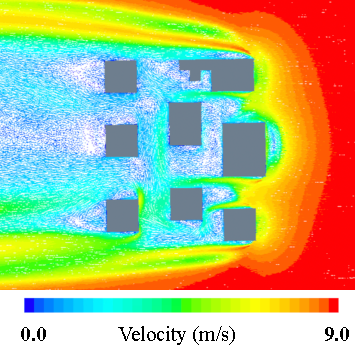
\includegraphics[scale=0.59]{fig10/CFD_map.pdf} &  \includegraphics[scale=0.6]{fig10/wind_N.pdf} \\
        \small \textcolor{red}{(a) The flow analysis through the CFD.} &
        \small \textcolor{red}{(b) The discretized wind map converted from the flow analysis of the CFD.} \\
    \end{tabular}
    \\~\\
    \textbf{Fig. 10.} \textcolor{red}{The wind map configuration for the optimization environment.}
    \label{fig: wind_map}
 \end{mdframed}     
    ~\\
    ~\pagebreak
    ~\\
   \textbf{We also modified Fig. 13 in the manuscript as follows (Page 13.)}\\
    \begin{mdframed}[ linewidth=.75pt, userdefinedwidth=0.9\textwidth]
    \begin{tabular}{m{0.3\textwidth}m{0.3\textwidth}m{0.3\textwidth}|}
    \includegraphics[scale=0.53]{fig13/wind_N.pdf}&
    \includegraphics[scale=0.57]{fig13/wind_NW.pdf}&
    \includegraphics[scale=0.57]{fig13/wind_SE.pdf}\\
    \small \textcolor{red}{(g) The discretized north direction wind map.} &
    \small \textcolor{red}{(h) The discretized north-west direction wind map.} &
    \small \textcolor{red}{(i) The discretized south-east direction wind map.} \\
    \end{tabular}
    ~\\
    ~\\
    \textbf{Fig. 13.} \textcolor{red}{Optimization result of two example cases (a-f) considering wind map derived by the inlet velocity with 9~m/s (g-i). 
    The drone travel in the SE direction between the two points that are at different altitudes.}
    \label{fig: wind_opt}
    %\end{figure*}
 \end{mdframed}       
	~\\
	~\\
    \item \textbf
    {
	C5: The DP algorithm was used for the optimization. The application of the algorithm is not clearly explained, which is necessary for the interested reader to know, and also for the replication. The DP algorithm comes with curse of dimensionality, and since the authors are dealing with a 3D case, it is very important to know the parameters used in DP algorithm for the optimization :~\\  
    Where is the DP algorithm running and how it connects with the drone?~\\
    It seems that the authors are interested in real-time application, in this case, why RTDP is not used? ~\\
    What are the computational costs of one DP sweep?~\\
    Computational complexity should also be shown based on the parameters used in the DP optimization, and how variation of the parameters effects the complexity of the algorithm?~\\
    Where is the optimization equation, along with optimization variable. The description of the model for DP algorithm should also be added.~\\
    How does the grid resolution effects the solution outcome and computational time?~\\
	}
	\item \textit
	{
	R5-1: We are thankful for the review of your kind advice. We agree that the information about DP should be useful to the reader. In this paper, we derive the drone's minimum energy path using the graph search algorithm in an offline manner at the base station and send the path to the drone to perform the optimal flight.
    We present the procedure of finding the drone's minimum energy path as Algorithm 2 in Subsection V-D.
    We also described the process of the optimal path planning in the graph line-by-line through the Dijkstra algorithm.
	}
	~\\
    \pagebreak ~\\
	\textbf{We added Algorithm~2 in the manuscripts as follows (Page 11.)}
	%\begin{mdframed}[ linewidth=.75pt, userdefinedwidth=0.9\textwidth]
    \SetNlSty{}{\color{red}}{:}
    \SetAlFnt{\color{red}}
%\noindent\begin{minipage}{.5\textwidth}    
    \RestyleAlgo{boxruled}
    \setcounter{algocf}{1}
    \begin{algorithm}[h]
    \caption{Problem procedure searching the energy optimal path of a drone.}
    \KwIn{\\
    %\textcolor{red}{
    \hskip1.5em $G$ // A created graph  \\
    \hskip1.5em $n_s$ // A source node  \\
    \hskip1.5em $n_d$ // A destination node 
    }
    \KwOut{\\
    \hskip1.5em $R$ // The minimum cost path from $n_s$ to $n_d$ \\
    \hskip1.5em $C$ // The cost of $R$
    }
    \nonl \hrulefill \\
    $reqCost$ := $\{\}$  \\
    $prevNode$ := $\{\}$ \\
    $Q$ := $priority\_queue()$ \\
    $reqCost[n_s]$ := 0 \\
    $prevNode[n_s]$ := $n_s$ \\
    \ForEach{$n_v$ in $G$}
    {
        \If{$n_v$ is not $n_s$}
        {
            $reqCost[n_v]$ := $\infty$ \\
            $prevNode$ := $None$
        }
        $Q.append(n_v, reqCost[n_v])$
    }
    \While{Q is not empty}
    {
	    $n_u$ := $Q.pop()$ \\
        \ForEach{neighboring node $n_w$ of $n_u$}    
        { 
    	    $cost$ := $reqCost[n_u]$ + $G.edgeWeight(n_u, n_w)$ \\
    	    \If{$cost$ $\leq$ $reqCost[n_w]$}
    	    {
    	        $reqCost[n_w]$ := $cost$ \\
    	        $prevNode[n_w]$ := $n_u$ \\
    	        $Q.modify\_priority(n_w, reqCost[n_w])$
    	    }
        }
    }
    $R$ := $[\ ]$ \\
    $C$ := $reqCost[n_d]$ \\ 
    \While{$n_d$ is not $n_s$}
    {
    $R.append(n_d)$ \\
    $d$ := $prevNode[n_d]$
    }
    \KwRet{$R$, $C$}
    \end{algorithm}
%\end{minipage}    
    \SetNlSty{}{\color{black}}{:}
    \SetAlFnt{\color{black}}
    %\end{mdframed}
    ~\\
    ~\\
    ~\\
    \pagebreak ~\\
	\textbf{We modified Section~VI in the manuscripts as follows (Page 11, Line ZZ.)}\\
    \begin{mdframed}[ linewidth=.75pt, userdefinedwidth=0.9\textwidth]
    \textcolor{red}{
    We present the procedure of finding the minimum energy optimal path of the drone in our configured problem as Algorithm 2 using the Dijkstra algorithm, which is a kind of the graph search algorithm\,[25], [26].
    Visiting each node of a graph is called traversal, and the Dijkstra algorithm, a traversal method, searches for the path that has the least weight from a source node to a destination node in the graph. The Dijkstra algorithm only can be used when the graph like $G$ that has no negative weight at the edge.
    As the input for solving the problem, we prepare a graph $G$, a source node $n_s$ where the drone starts the mission, and a destination node $n_d$ representing the destination of the task.
    The variable $reqCost$ stores cost from the source node to arbitrary nodes in $G$ and $prevNode$ stores the predecessor that has the smallest $cost$ among the connected nodes of the current node (Line 01,02). 
    Note that the cost is calculated as the required energy to travel between nodes by using the drone power model in Section~V.
    The Dijkstra algorithm uses a priority queue instead of a normal queue and searches for the shortest path relatively quickly compared with the breadth-first search and depth-first search.
    Thus, the Dijkstra algorithm finds the energy optimal path (the shortest path) between $n_s$ and $n_d$.}~\\
    \textcolor{red}{Each element of the priority queue has a priority, so elements with higher priority are processed before elements with lower priority.
    We declare $Q$ as the priority queue as a binary min-heap and initialize $Q$ by calling all nodes of $G$ (Line 03).
    We append arbitrary node $n_v$ to $Q$ with a priority of infinity (Line 06). 
    At this time, the priority of the source node $s$ is initialized to 0.
    After that, the highest priority node $n_u$ is selected from the $Q$. 
    In Algorithm 2, we use the weight of an edge as a priority.
    We obtain $cost$ which is a sum of $reqCost$ of $n_u$ and the calculated cost between $n_u$ and each neighbor node $n_w$ using~(6.2) (Line 13). 
    Then, we compare $cost$ with the stored $reqCost$ in $n_w$.
    When $cost$ is smaller than $reqCost$, $prevNode$ of $n_w$ is updated to $n_u$, and the priority of $n_w$ in the queue is updated to $cost$ (Line 18).
    The process continues until $Q$ becomes empty.
    We set $R$ as a list for storing the shortest path between $n_s$ and $n_d$ along $prevNode$.
    We record the minimal cost information in $C$ to need the moving from $n_s$ to $n_d$ along with the stored node of $R$ (Line 21).
    }
    \end{mdframed} 
    ~\\
	\item \textit
	{
	R5-2: RTDP~[4] searches the optimal velocity for each step of the discretized environment in the local solution space. %However, the sequence of the optimum velocity chosen for local spaces through RTDP may not be globally optimal in the overall environment.
	There are problems with the computational cost of online planning. Since, the drone’s onboard computer is not suitable for computing complex algorithms. Even if the complex computation that is solved externally is sent to drones in real-time, the drone requires additional cost for long-distance communications. The time racks that occur during long-distance communication also increase the power consumption of drones.
	~\\
	~\\
    Our research is to reduce the energy consumption of the drone without significant hardware improvements. The online planning method is not suitable for us.
    Instead of online planning, we have created an optimization environment similar to reality.
    Under the assumption that there is no sudden accident (e.g., bird strike), we present the method that transmits the optimal path derived by the base station that computes complex computation to the drone to reduce the drone's energy consumption.
	}
	~\\
	\item \textit
	{
	R5-3: The Dijkstra algorithm requires the RAM capacity as much as the size of the graph, and the computational cost depends on the grid resolution of our environment.
    Our one DP sweep in the simulation is to explore the minimum energy path from the start node to the destination node. It takes less than half of a second.
	}
	~\\
	\item \textit
	{
	R5-4: Our parameters of the algorithm are factors comprising the node $n_i$ (6.1), and we determine the number of nodes $N_n$ by the number of steps per each parameter in the environment. 
    All nodes of the graph are initially stored in the priority queue. Then, the algorithm modifies the priority of neighboring nodes of every node in the priority queue, requiring $N_e$ iterations. Therefore the time complexity of the algorithm is $O(N_e log(N_n))$ since the time complexity of modifying the priority is $O(log(N_n))$.~\\
    To reduce the number of node, we apply the heuristic that the backward directions that drone can move are excluded as we described in Section~VI.
    \\
    \\
    When the number of nodes and edges changes according to the change of the parameter of the algorithm, the computational cost changes, but it does not affect the time complexity.
    We present the information about the Dijkstra algorithm in Subsection VI-D.
	}
	~\\
    ~\\
	\textbf{We modified Section~VI in the manuscripts as follows (Page 11, Line ZZ.)}\\
    \begin{mdframed}[ linewidth=.75pt, userdefinedwidth=0.9\textwidth]
    \textcolor{red}{
    The algorithm parameters are the number of nodes, and we determine the number of nodes $N_n$ by the number of steps per each parameter in the environment.  
    We set the range of coordinate information in the node to 20 steps of 20\,m each for the N-axis and E-axis, 20 steps of 3\,m for the U-axis, and also set the range of drone speed to 7\,steps of 2\,m/s. 
    The wind map has a speed range of up to 9\,m/s with eight directions.
    The process of modifying the priority of all nodes in $Q$ has a time complexity of $log(N_n)$, where $N_n$ stands for the number of nodes.
    Repeating until $Q$ is empty, each node searches their neighbor nodes, so $log(N_n)$ is repeated as many as the number of edges, where $N_e$ is the total number of edges in $G$. 
    Thus, the algorithm has the following time complexity.~\\
    \begin{equation*}
    O(N_elog(N_n)) \tag{6.3} \label{eq:complexity}
    \end{equation*}~\\
    When the number of nodes and edges changes according to the change of the parameter of the algorithm, the computational cost changes, but it does not affect the time complexity.
    }
    \end{mdframed} 
    ~\\
	\item \textit
	{
	R5-5: We formulate our optimization problem and describe it in the additional Subsection of Section VI. We present the scenario for the optimization process of the drone in Fig.8 and variables for optimization into Given, control knob, and objective.~\\
    In our optimization problem, the workspace $W$ where the drone is operated, the wind information $F$ in the horizontal directions provided through the discretized wind map, and the information of obstacles in the environment $BL$ are $Given$ information.
    The starting point and destination of the mission, and information of the payload are also $Given$ information.~\\
    We define the function $Path$ using $w$ within the $W$ and the velocity of the drone $v$ as $R$, and we use the function $Path$ as our control knob.
    Our objective is to find $Path$ that minimizes the function $E$ of the energy through the optimization process when a base station receives the mission $m$ from a drone.
    The energy function $E$ cannot exceed the initial battery capacity, $BL$ must be zero for all $w$, and $Path$ consists only of $w$ presented in $W$.~\\
    Our model for the algorithm is the function of $E$, which is the total energy consumption for the delivery mission.
	}
	~\\
	~\\
	\textbf{We added newly Subsection~VI-C in the manuscripts as follows (Page 08, Line ZZ.)}\\
    \begin{mdframed}[ linewidth=.75pt, userdefinedwidth=0.9\textwidth]
    \textbf{\justify\textcolor{red}{A. Problem formulation}}~\\
    ~\\
    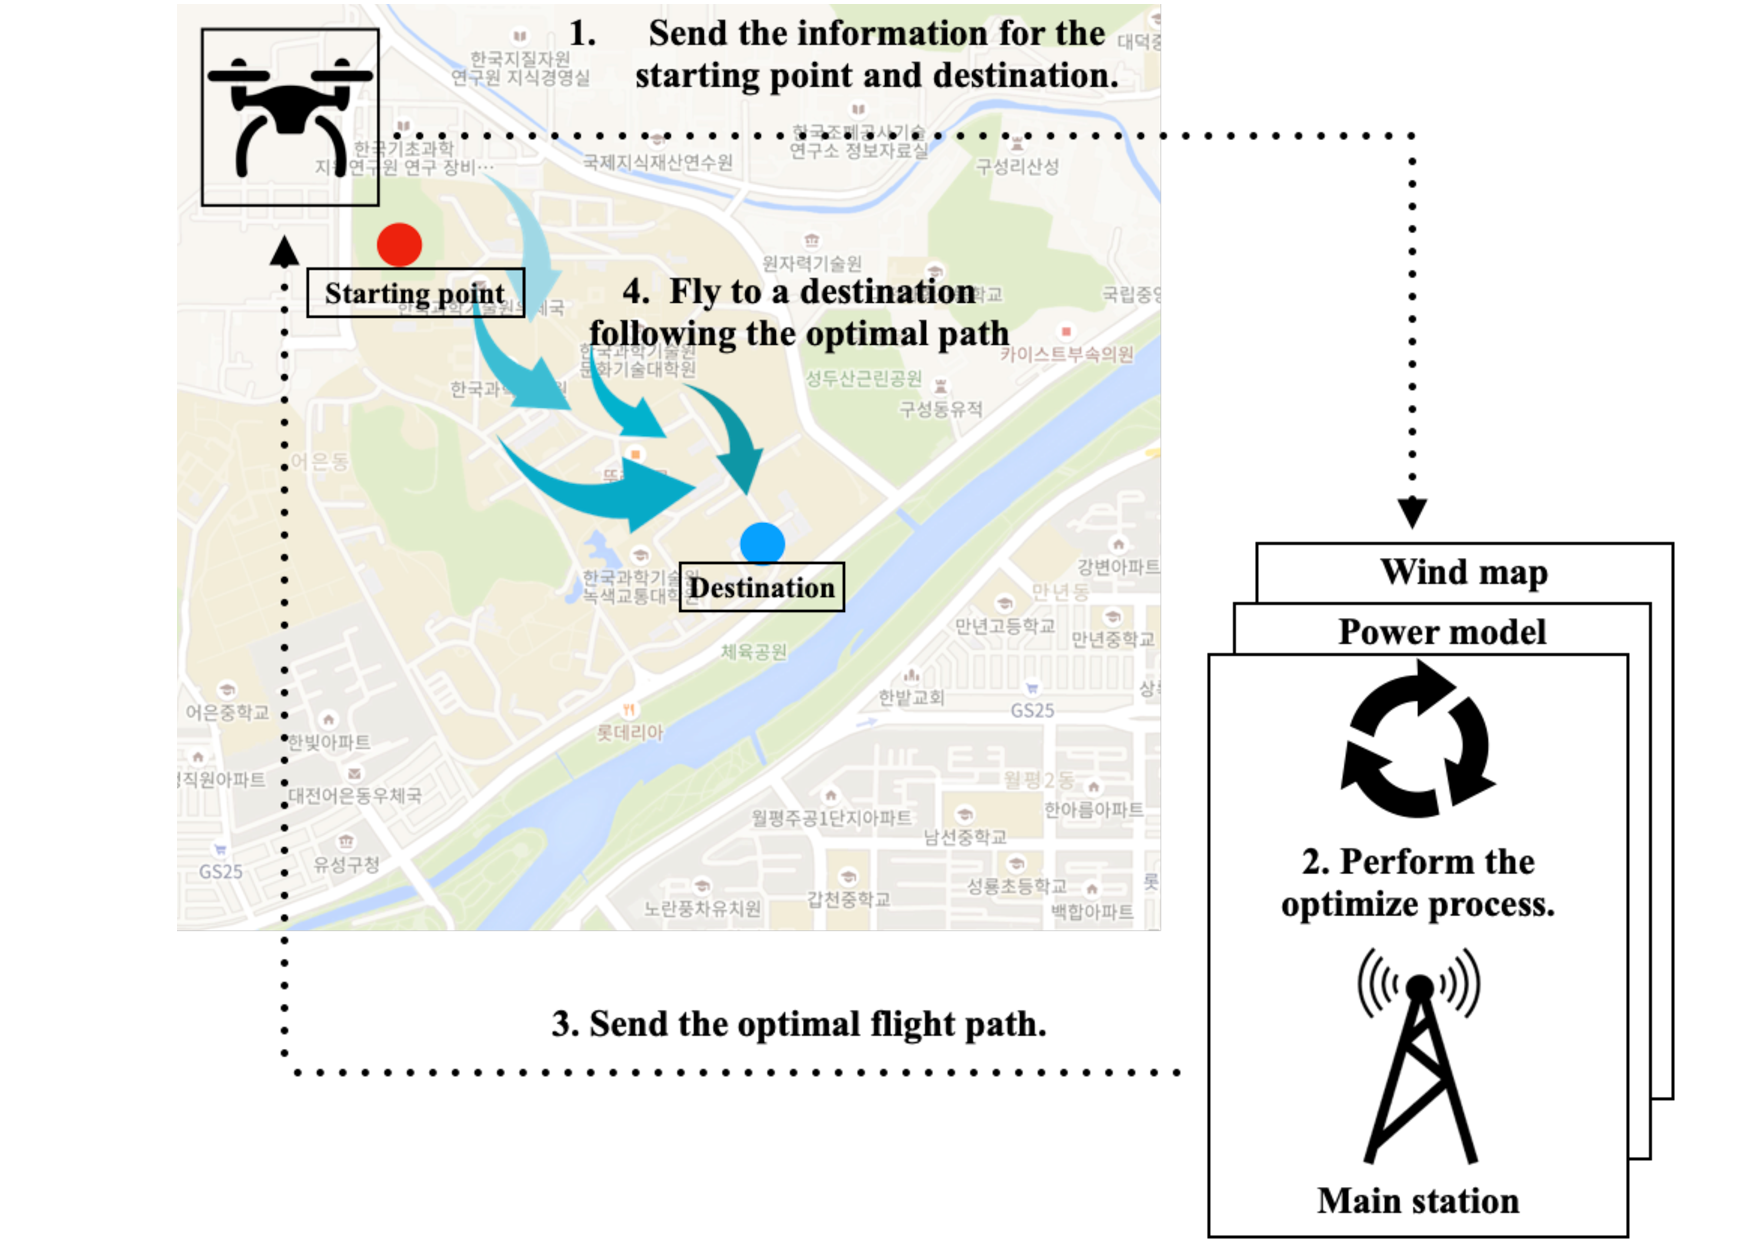
\includegraphics[scale=0.34]{fig8/problem_formulation.pdf}~\\
    \textcolor{red}{Fig. 8. The scenario of the drone optimization process.}~\\
    \justify\textcolor{red}{In our scenario, the operator inputs information about a starting point and a destination to the main station to assign a task to the drone, as shown in Fig.\,8.
    The station holds the power consumption model of the drone and wind maps about the operating environment, and the station derives the path between points entered from the operator.
    % Offline 최적화임을 여기서 언급
    Since the optimization is performed offline at the main station, it is impossible to modify the optimal path already drawn while the drone is running. Also, in this paper, we do not assume that the station considers the unexpected situations such as bird-strike or wind-sheer.
    % 외부 바람을 고려하기 위해 전용 툴을 쓴다는 것을 여기서 언급함
    However, we analyze the predictable external forces such as wind level and direction using the sophisticated analysis tool to take full advantage of the effects of external forces in creating the optimal path of the drone. 
    After that, the drone receives the optimized path from the station and then runs to the destination along the path. We formulate the flight energy optimization problem of the drone as the following:}

    \textcolor{red}{
    \vspace{7pt}
    \hrule
    \vspace{5pt}
    \noindent\textit{\textbf{Flight energy optimization problem formulation}}
    \vspace{5pt}
    \hrule
    \vspace{5pt}
    \noindent Workspace $W$ is a subset of $\mathbb{R}^3$ that drones can maneuver, and $F(\cdot)$, $B(\cdot)$ take the $W$ as the domain:\\
    \indent Workspace, \textit{$W\subset\mathbb{R}^3$, $w_n=(x_n,y_n,z_n)$, $w_n \in W$ }\\
    \indent Blockage, \textit{$BL(w_n)=bl_n$}, while blockage $bl_n\in\{0,1\}$\\
    \indent Wind field, \textit{$F(w_n) = (windx_n, windy_n)$}, while $windx_n$ is  
     x-axis wind velocity and $windy_n$ is y-axis wind velocity
     at $w_n$, respectively.
    \vspace{5pt}
    \hrule
    \vspace{5pt}
    \noindent\textit{\textbf{Given:}}~\\
    \indent $W, F(\cdot), BL(\cdot)$~\\
    \indent Set of delivery missions, $M = \{m_1, ..., m_J\},$~\\ 
    \indent $m_j = (from, to, package\;volume, package\;weight)$~\\
    \noindent\textit{\textbf{Control knob:}}~\\
    \indent Path, finite sequence of $(w,v)$,~\\
    \indent $R = \{(w_0,v_0), ..., (w_N,v_N)\}$, while $v$ is a velocity vector.
   ~\\
    \noindent\textit{\textbf
    {Objective:}}~\\ 
    \indent Minimize total consumption energy~\\
    \indent\indent $\sum_{j=1}^J E(m_j,R_j)$,~\\
    \indent while $E$ is energy consumption for the delivery mission $m_j$ through a path $R_j$, which satisfies~\\
    \indent\indent $BL(w_n) = 0, \forall w_n \in \bigcup_{1}^J R_j,$~\\
    \indent\indent $E(m_j, R_j) \leq$ Initial battery capacity.
    \vspace{5pt}
    \hrule
    \vspace{5pt}
    }
    \vspace{5pt}
    
    \textcolor{red}{In our optimization problem, the workspace $W$ where the drone is operated, the wind information $F$ in the horizontal directions provided through the discretized wind map, and the information of obstacles in the environment $BL$ are $Given$ information.
    The starting point and destination of the mission, and information of the payload are also $Given$ information.
    We define the function $Path$ using $w$ within the $W$ and the velocity of the drone $v$ as $R$, and we use the function $Path$ as our control knob.
    Our objective is to find $Path$ that minimizes the function $E$ of the energy through the optimization process when a base station receives the mission $m$ from a drone.
    The energy function $E$ cannot exceed the initial battery capacity, $BL$ must be zero for all $w$, and $Path$ consists only of $w$ presented in $W$.}
    \end{mdframed}
    ~\\
    ~\\
	\item \textit
	{
	R5-6: The number of nodes and edges varies depending on the grid resolution, and we conducted the computation for the path optimization of the drone using all of the computational resources available to us. When the number of nodes and edges increases with the high grid resolution, we can further refine the parameters that the nodes contain to improve the accuracy of energy consumption prediction or to optimize the drone’s path planning on a broader environment.
    If the number of nodes and edges decreases with the low grid resolution, we can optimize the drone’s path planning in less time instead of sacrificing the accuracy of the energy consumption prediction.
	}
	~\\
    ~\\
    \textbf{We modified Section~VI in the manuscripts as follows (Page 12, Line ZZ.)}\\
    \begin{mdframed}[ linewidth=.75pt, userdefinedwidth=0.9\textwidth]
    \textcolor{red}{
    The number of nodes and edges varies depending on the grid resolution, and we conduct the computation for the path optimization of the drone using all of the computational resources available to us. When the number of nodes and edges increases with the high grid resolution, we can further refine the parameters that the nodes contain to improve the accuracy of energy consumption prediction or to optimize the drone’s path planning on a broader environment.
    If the number of nodes and edges decreases with the low grid resolution, we can optimize the drone’s path planning in less time instead of sacrificing the accuracy of the energy consumption prediction.}
    \end{mdframed} 
    ~\\
    \item \textbf
    {
	C6: Graph search: \\
	``The acceleration of the drone uses the maximum acceleration the drone can exert, and increases linearly'' If the maximum acceleration is used, then what is increasing?	
	}
	\item \textit
	{
	R6: We sincerely apologize for the error in the sentence. when a drone moves from an arbitrary node in $G$ to adjacent nodes there are two patterns of speed change. When the drone accelerates, it moves its current velocity until the end then it accelerates to the target velocity of an adjacent node. 
    In the case of the deceleration, the drone moves at a constant velocity toward the adjacent node, then it decelerates to the instantaneous velocity that satisfies an adjacent node to reach the target node.
    Since the continuous changes in the velocity and acceleration of the drone cannot be calculated in the discretized environment, we calculate the instance power at each node then we apply the averaged power along traveling two nodes.
%	Since the continuous changes in the velocity and acceleration of the drone are not considered in the discretized environment, we assume that the acceleration and velocity of the drone while moving are the average value between the two nodes.~\\
    %In Algorithm~1, We denote $\Delta t_1$ as the required time for acceleration or deceleration. 
    %It is obtained by dividing the velocity difference ($V_n - V_c$) between the current node $n_c$ and the adjacent node $n_n$ by the acceleration in the drone's moving direction.~\\
    %At this time, the drone's horizontal acceleration is $A_h$, and vertical acceleration is $A_v$. We assume that the drone accelerates with its maximum acceleration. For the target drone M600, the horizontal acceleration is $5~m/s^2$ and vertical acceleration is $1~m/s^2$, respectively.~\\
    %We corrected Heuristic 2, which contained incorrect sentences, and we explained the process for considering acceleration in the graph search algorithm in Subsection VI-C.
	}
	~\\
	~\\
	\textbf{We modified Section~VI in the manuscripts as follows (Page 10, Line ZZ.)}\\
    \begin{mdframed}[ linewidth=.75pt, userdefinedwidth=0.9\textwidth]
    Heuristic 2. \textcolor{red}{About t}he instantaneous velocity at the next node: \textcolor{red}{During the traveling, the drone first accelerates to the target velocity if it is necessary. Then, it moves the remaining distance with constant velocity. In case of the deceleration, the drone moves constant velocity. Then it decelerates to the target velocity lastly.}
    \end{mdframed} 
    ~\\
    ~\\
    %~\\ \pagebreak ~\\
    \textbf{We also modified Section~VI in the manuscripts as follows (Page 10, Line ZZ.)}\\
    \begin{mdframed}[ linewidth=.75pt, userdefinedwidth=0.9\textwidth]
\textcolor{red}{In Algorithm 1, when a drone moves from an arbitrary node in $G$ to adjacent nodes there are two patterns of speed change. When the drone accelerates, it moves its current velocity until the end then it accelerates to the target velocity of an adjacent node (Line 08).}
\end{mdframed}
~\\~\\
    \item \textbf
    {
	C7: Experimental results: \\
	This section starts abruptly, without giving any information regarding the experimental methodology. It seems to me that this is a simulation based test, however it should be clearly written.~\\
	The optimization algorithm, if applied on the drone in simulation, then where are the drone parameters, how did you obtain them?~\\
	which simulation tool you have used. What are the computational costs of running the optimziation algorithm. Computational costs or calculation time, is specially important,~\\
	if you are developing a real-time optimization tool. It would also be very interesting to know the power output for all cases, along with the traversed path.
	}
	~\\
	~\\
	\item \textit
	{
	R7-1: We sincerely apologize less information regarding the methodology. We deeply agree that the experiment section should give enough information to readers. When we configure the environment for the optimization, we store the three-dimensional coordinates and drone parameters on the graph. The node $n_i$ in the graph is defined as (6.1).
    \begin{equation*}
    n_i = (x_i, y_i, z_i, v_i, a_i, w_i, d_i). \tag{6.1} \label{eq:node}
    \end{equation*}
    The algorithm parameters are the number of nodes, and we determine the number of nodes $N_n$ by the number of steps per each parameter in the environment. 
    We also explained how the graph search algorithm applied to our optimization problem with Algorithm 2 and Subsection VI-D (R5-1).
	}
	~\\
	\item \textit
	{
	R7-2: We conducted the simulation using the matlab of Mathwork. Our computational cost is the amount of RAM in the size of a graph to create an optimization environment. We determine the number of nodes by the number of steps per each parameter in the environment. We wrote the range of the node’s parameters in Subsection VI-D.~\\
    In addition, we create a graph from the optimization environment, and we use the graph search algorithm to find the optimal path for the drone. However, it takes a lot of time to generate a graph, and we assume that the base station already has a large number of graphs that have been created considering the varying environmental conditions. It takes 10 seconds to get the environment graph into the matlab and about 0.5 seconds to find the optimal path on the graph. We wrote the above in Section VI.
	}
	~\\
	~\\
	\textbf{We modified Section~VI in the manuscripts as follows (Page 11, Line ZZ.)}\\
    \begin{mdframed}[ linewidth=.75pt, userdefinedwidth=0.9\textwidth]
    \textcolor{red}{The algorithm parameters are the number of nodes, and we determine the number of nodes $N_n$ by the number of steps per each parameter in the environment.  
    We set the range of coordinate information in the node to 20 steps of 20\,m each for the N-axis and E-axis, 20 steps of 3\,m for the U-axis, and also set the range of drone speed to 7\,steps of 2\,m/s. 
    The wind map has a speed range of up to 9\,m/s with eight directions.
    }
    \end{mdframed} 
    ~\\
	\textbf{We modified Section~VI in the manuscripts as follows (Page 11, Line ZZ.)}\\
    \begin{mdframed}[ linewidth=.75pt, userdefinedwidth=0.9\textwidth]
    \textcolor{red}{It takes about 2 hours to generate $G$ under the Intel® i7-8086K CPU @ 4.00 GHz (12 cores), 32 GB 2400 MHz DDR4 RAM using MATLAB of MathWorks®. 
    However, if the main station already has a large number of graphs created in consideration of environmental changes, the computational time at the station is less than 0.5 seconds to find the optimal path. The appropriate graph should be loaded into the RAM before it starts to find the optimal path. Note that to load a pre-processed graph into the RAM takes about 10 seconds whenever the drone executes missions.
    }
    \end{mdframed} 
    ~\\
    ~\\
	\item \textit
	{
	R7-3: Although we do not proceed with online planning, the edge selected by the Dijkstra algorithm has the smallest energy consumption compared with all the edges connected to the same node, and the derived path is the optimal solution in the discretized environment.
    Instead of online planning, we chose to improve the environment for the optimization, and we presented Table IV as a result of the optimization. 
	}
	~\\
	~\\
	\textbf{We added Table~IV in the manuscripts as follows (Page 14.)}\\
%    \begin{table*}[!h]
    \begin{mdframed}[ linewidth=.75pt, userdefinedwidth=0.9\textwidth]
    \textcolor{red}{\textbf{Table IV.} Comparison of the energy consumption between the baseline and the optimal path affected by wind effect in each case.}   
%    \caption{}
    \centering
    \label{tab: opt.result}
    %\resizebox{\textwidth}{!}{%
    \textcolor{red}{
    \begin{tabular}{|c|c|c|c|c|c|c|}
    \hline
    \multirow{2}{*}{} & \multirow{2}{*}{Wind map} & \multicolumn{2}{c|}{Energy consumption (kJ)} & \multicolumn{2}{c|}{Travel time (sec)} & \multirow{2}{*}{Saved energy (\%)} \\ \cline{3-6}
                        &            & Baseline & Optimal path & Baseline               & Optimal path &      \\ \hline
    \multirow{2}{*}{Case 1} & Fig. 13(i) & 38.1     & 36.2         & \multirow{2}{*}{44.10} & 40.84        & 5.27 \\ \cline{2-4} \cline{6-7} 
                        & Fig. 13(g) & 46.3     & 45.4         &                        & 46.53        & 1.8  \\ \hline
    \multirow{2}{*}{Case 2} & Fig. 13(i) & 44.7     & 43.9         & \multirow{2}{*}{53.58} & 50.68        & 1.9  \\ \cline{2-4} \cline{6-7} 
                        & Fig. 13(h) & 45.7     & 45.4         &                        & 52.33        & 0.7  \\ \hline
    \end{tabular}%
    }
    %}
    %\end{table*}
    \end{mdframed}
    ~\\
    ~\\
    \item \textbf
    {
	C8: Language, grammar and presentation: \\
	Reviewer recommends a thorough proofread for occasional but important language problems.
	The use of articles is sometimes not correct, some examples are: ``Finally, we demonstrate a example of energy saving by finding an energy efficient path during the operation of a drone using the proposed accurate power consumption model.'' it should be ``we demonstrate an example''
	}
	\item \textit
	{
	R8: We sincerely apologize for many grammar errors. We carefully double-checked the manuscript and fully revised sentences. We denoted changed sentences as red color. We appreciate your invaluable comments.
    }
    ~\\
    \item \textbf
    {
	C9: An example of incorrect capitalization is: \\
	``In order to construct the Accurate power consumption model based on the actual drone data, we figure out the power consumption characteristics of a top-of-the-line commercial drone through dozens of hours of power measurement both on the air and ground.'', Accurate $\rightarrow$ accurate
	``Case 2. The wind speed of 6 m/s are
	applied in the NW and SE directions to the operation environment, respectively. but, The drone travel in the SW direction between the two points that are at different altitudes.'' Please check the sentence punctuation and for grammar.
	SI units should be used, for instance change (sec) to (S)
	Please check the latex code for the Algorithm 1. It can be better, for instance, adding vertical lines showing the loops or if else conditions.
	Furthermore, the caption can be enclosed by line above and below and a line below the algorithm 1.
	}
	\item \textit
	{
	R9: 그림 수정이 필요하여 잠시 비워두었습니다. (주중에 채워놓겠습니다.)
    }
    ~\\
	~\\
	\textbf{We modified Section~VI in the manuscripts as follows (Page 12, Line ZZ.)}\\
    \begin{mdframed}[ linewidth=.75pt, userdefinedwidth=0.9\textwidth]

    \end{mdframed} 
    ~\\
	~\\
	\textbf{We modified Section~VI in the manuscripts as follows (Page 12, Line ZZ.)}\\
    \begin{mdframed}[ linewidth=.75pt, userdefinedwidth=0.9\textwidth]

    \end{mdframed} 
    ~\\
	~\\
	\textbf{We modified Section~VI in the manuscripts as follows (Page 12, Line ZZ.)}\\
    \begin{mdframed}[ linewidth=.75pt, userdefinedwidth=0.9\textwidth]

    \end{mdframed} 
	~\\
    ~\\
\end{description}

\textbf{\large Reviewer 4:}\\
This manuscript presents a deep-neural-network-based approach to model the energy consumption in terms of motion parameters of a multi-copter and a path-planning algorithm that minimizes the energy consumption given a predefined starting and ending points. An off-the-shelf multi-copter was adopted to validate some aspects of the proposed methodology.  Please see the detailed comments below. 
\begin{description}
    \item \textbf
	{
	C1: The expression of the manuscript at many places is confusing. For example, “…if the collected amount of data is a lot and accurate enough…”, just to name one. The authors are strongly suggested to polish the English writing.  A professional copy editor would be a good option..
	}
	\item \textit
	{
	R1: We sincerely apologize for many grammar errors. We carefully double-checked the manuscript and fully revised sentences. We denoted changed sentences as red color. We appreciate your invaluable comments.  
	}
	~\\
    ~\\
    \item \textbf
    {
	C2: The literature review is well done, while considering the length of the paper, it is suggested shorten the Introduction and Related Work sections.
	}
	\item \textit
	{
	R2: We really appreciate your encouraging comment. We summarized Section I and Section II after adding two papers to our reference that appropriate the current trend at the request of another reviewer.
	}
	~\\
    ~\\
	\textbf{We added References as follows (Page 14, Line ZZ.)}
    \begin{mdframed} [ linewidth=.75pt, userdefinedwidth=0.9\textwidth]
    \textcolor{red}{[4] Abdullah Mohiuddin, Tarek Taha, Yahya Zweiri, and Dongming Gan. Uav payload transportation via rtdp  based optimized velocity profiles. Energies, 12(16):3049, Aug 2019.} \\
    \textcolor{red}{[13] S. Shin, Y. Kang, and Y. Kim. Automatic drone navigation in realistic 3d landscapes using deep reinforcement learning. In 2019 6th International Conference on Control, Decision and Information Technologies (CoDIT), pages 1072–1077, 2019.}
    \end{mdframed} 
    ~\\
    ~\\
	\textbf{We modified Section~II in the manuscript as follows (Page 2, Line ZZ.)}
    \begin{mdframed} [ linewidth=.75pt, userdefinedwidth=0.9\textwidth]
    \textcolor{red}{A. Mohiuddin~et~al focus on the real-time optimization of the drone\,[4]. 
    The authors infer the optimal velocity of the drone to proceed to the next states based on the current state of the drone as an agent in the environment.
    They predict the power consumption of the drone through the dynamics-based power consumption model and optimal velocity inferred by the real-time dynamic programming.
    Reinforcement learning is one of the optimization solutions\,[13].
    They focus on solving the task problem of the drone in the partially observable Markov decision process. They utilize Convolutional neural networks that use convolutional filters to detect edges of the picture taken by the drone and extract the characteristics of the image, and they predict the best action at each step in the discretized environment using Double deep Q networks.}
    \end{mdframed}   
	~\\
    ~\\
    \textbf{We also modified Table~I in the manuscript as follows (Page 3.)}
    \begin{mdframed} [ linewidth=.75pt, userdefinedwidth=0.9\textwidth]
    \textbf{Table I Comparison of previous works for \textcolor{red}{the} drone optimization.}
    \centering
    \resizebox{.95\textwidth}{!}{
    \begin{tabular}{|c|c|c|c|c|c|}
    \hline
    Reference & Wind & Payload & Surface area & Optimization method & Goal \\ \hline
    %TVLSI 2019 & \cmark & \cmark & \cmark & Dijkstra algorithm & \multicolumn{1}{l|}{Minimum energy} \\ \hline
    ICARSC 2015~[10] & %\xmark 
    & %\xmark 
    & %\xmark 
    & Back-and-forth algorithm & Minimum energy \\ \hline
    IROS 2016~[6] & \cmark & %\xmark 
    & %\xmark 
    & Model predictive control & Minimum energy \\ \hline
    ICRA 2016~[8]  & %\xmark 
    & \cmark & %\xmark 
    & SQP algorithm & Minimum energy \\ \hline
    IMAV 2017~[9] & %\xmark 
    & \cmark & \cmark & LGR orthogonal collocation & Minimum energy \\ \hline
    SysCon 2017~[12] & \cmark & %\xmark 
    & %\xmark 
    & Fast marching method & Minimum energy \\ \hline
    arXiv 2017~[11] & \cmark & \cmark & %\xmark 
    & Dynamic graph algorithm & Shortest time \\ \hline
    \textcolor{red}{CoDIT 2019 {[13]}} &  &  & %\xmark 
    & \textcolor{red}{Reinforcement learning} & \textcolor{red}{Shortest time} \\ \hline
    \textcolor{red}{Energies 2019 {[4]}} & \textcolor{red}{\cmark} & \textcolor{red}{\cmark} 
    & \textcolor{red}{\cmark} & \textcolor{red}{Real-time dynamic programming} & \textcolor{red}{Minimum energy} \\ \hline
    \end{tabular}
    }
    \end{mdframed} 
    ~\\	
    ~\\
    \item \textbf
    {
	C3: It is unclear how wind speed knowledge is used in modeling and path-planning optimization. As stated in Section IV.D, the wind sensor was used to collect real-time wind data, but in Section VII, it says that “there is no way to receive wind data in real-time”. 
	}
	\item \textit
	{
	R3: In the modeling process, the wind affects a significant influence on the drone’s power consumption. Therefore, when constructing the power consumption model, we installed a wind sensor on the drone, collected the wind data in real-time, included those data into a learning dataset to model the power consumption.
    Apart from the modeling, in the optimization process, the online planning involves several problems using wind data as a parameter.
    ~\\
    ~\\
    First of all, the more parameters to consider in the optimization, the more complex the optimization problem becomes. The on-board computer of the drone is not suitable for handling huge computations in real-time.
    Secondly, even if the drone receives the computation results that are solved externally, the drone must deliver wind information to the server for the calculation in real-time , the drone requires additional cost for long-distance communications. 
    Moreover, Our research is to reduce the energy consumption of the drone without significant hardware improvements. The online planning method is not suitable for us.~\\
    However, offline planning also requires to know the direction and the speed of the wind at every grid cell of the simulation environment. In order to derive the optimal path for reality, the simulation environment must also be as similar as possible to the actual conditions.
    ~\\
    ~\\
    So, we used the computational fluid dynamics (CFD) to interpret the flow in our simulation environment, and to adapt it to our grid resolution, we made it in the form of a discretized wind map to enhance our simulation environment close to reality.
    We explained the CFD and wind maps in Subsection VI-B and presented the Fig.13 of wind maps used in simulation in Subsection VII-B.
	}
	~\\
    ~\\
	\textbf{We modified Section~VI and added Fig. 10 in the manuscripts as follows (Page 09, Line ZZ.)}\\
    \begin{mdframed}[ linewidth=.75pt, userdefinedwidth=0.9\textwidth]
    \justify
    \textcolor{red}{The wind velocity is a crucial factor that significantly affects the power consumption of the drone. Let us assume that the wind is measured with a dedicated expensive sensor by the drone in real-time. There would be a long process occurs; 
    the drone measures the wind for each step, transmits the information to a station far away, and transmits the movement corresponding to the next step derived from the station back to the drone.
    During the process, the time lag generated by the calculation time for optimization in each step affects the optimal operation of the drone. 
    Also, long-distance communication between the drone and station also consumes the computational and power cost of the drone.
    Unless the user measures wind directly from the drone, there are very limited methods for obtaining wind information (for example, receiving the data from the meteorological agency).
    In order to overcome these difficult conditions, we use a method to create a wind map through the CFD so that we can consider the effects of wind on drones in offline optimization.
    Computational fluid dynamics (CFD) uses computers to simulate the interaction of fluids and gases in engineering problems\,[24]. 
    The CFD converts the Navier-Stokes Equations, which are nonlinear partial differential equations describing fluid phenomena, into algebraic equations, and solves and analyzes fluid flow problems using algorithms of numerical techniques.
    We build wind map from the average wind speed data provided by the meteorological agency for the drone operation through the flow analysis using the CFD and store them for each wind speed wind direction, as shown in Fig.\,10(a).}~\\
    \noindent\textcolor{red}{
    We only use the horizontal wind velocity analyzed through CFD at each step of the height axis except for the influence of the pure vertical wind since the drone power consumption model only includes the horizontal wind velocity, which is directly measured by the wind sensor attached to the drone. 
    We assume that the effect of the pure vertical wind on the drone is excluded as mentioned in Section IV.
    We convert the analyzed wind data through CFD to the discretized wind map like Fig.10(b) and make it possible to match the three-dimensional coordinate information of the graph with the wind velocity of the discretized wind map.
    %The wind map contains the flow phenomena that occur when each direction of the wind from the inlet to an intensity of 9 m/s meets obstacles.
    We build various wind maps by changing inlet wind directions.}
    After that, \textcolor{red}{we use wind maps} as a lookup table so that the optimal route of the drone could be searched offline without \textcolor{red}{measuring} the wind directly from the drone.
    \\~\\
    %\begin{figure}[h]
    ~\par
    \centering
    \setcounter{figure}{9}
    %\subfloat[
    %]
    \begin{tabular}{m{0.45\textwidth}m{0.45\textwidth}}
        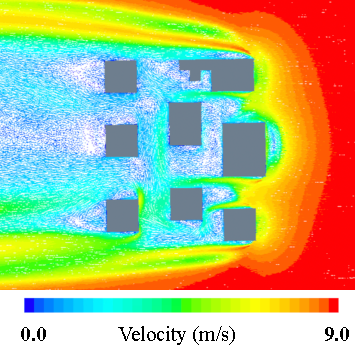
\includegraphics[scale=0.59]{fig10/CFD_map.pdf} &  \includegraphics[scale=0.6]{fig10/wind_N.pdf} \\
        \small \textcolor{red}{(a) The flow analysis through the CFD.} &
        \small \textcolor{red}{(b) The discretized wind map converted from the flow analysis of the CFD.} \\
    \end{tabular}
    \\~\\
    \textbf{Figure 9.} \textcolor{red}{The wind map configuration for the optimization environment.}
    \label{fig: wind_map}
    %\end{figure}
 \end{mdframed}     
    ~\\
    ~\pagebreak ~
    ~\\
    \textbf{We also modified Fig. 13 in the manuscript as follows (Page 13.)}\\
    \begin{mdframed}[ linewidth=.75pt, userdefinedwidth=0.9\textwidth]
    \begin{tabular}{m{0.3\textwidth}m{0.3\textwidth}m{0.3\textwidth}}
    \includegraphics[scale=0.53]{fig13/wind_N.pdf}&
    \includegraphics[scale=0.57]{fig13/wind_NW.pdf}&
    \includegraphics[scale=0.57]{fig13/wind_SE.pdf}\\
    \small \textcolor{red}{(g) The discretized north direction wind map.} &
    \small \textcolor{red}{(h) The discretized north-west direction wind map.} &
    \small \textcolor{red}{(i) The discretized south-east direction wind map.} \\
    \end{tabular}
    ~\\
    ~\\
    \textbf{Fig. 13.} \textcolor{red}{Optimization result of two example cases (a-f) considering wind map derived by the inlet velocity with 9~m/s (g-i). 
    The drone travel in the SE direction between the two points that are at different altitudes.}
    \label{fig: wind_opt}
    %\end{figure*}
 \end{mdframed}       
	~\\
	~\\
    \item \textbf
    {
	C4: Since the graph search algorithm has been used extensively in the proposed methodology, it would be helpful to present a summary of this algorithm and explain how it was applied. 
	}
	\item \textit
	{
	R4: We appreciate your invaluable comment. We also agree with the reviewer's comment that the explanation of the algorithm would be helpful for readers. We enhance the description of the algorithm as follows: 
	~\\
	~\\
	When we configure the optimization environment, we store the three-dimensional coordinates and drone parameters on the graph. 
    The node $n_i$ in the graph is defined as (6.1).
    \begin{equation*}
    n_i = (x_i, y_i, z_i, v_i, a_i, w_i, d_i). \tag{6.1} \label{eq:node}
    \end{equation*}
    Visiting each node of a graph is called traversal, and the Dijkstra algorithm, a traversal method, searches for the path that has the least weight from a source node to a destination node in the graph. The Dijkstra algorithm uses a priority queue instead of a normal queue and searches for the shortest path relatively quickly compared with the breadth-first search and depth-first search. The Dijkstra algorithm selects a node from the queue and searches all adjacent nodes to adjust the priority. When searching all queues, select the edge with the smallest cost and infers the optimal energy path.
    We presented the procedure of finding the drone's minimum energy optimal path in our configured problem as Algorithm 2, and we explained the algorithm line-by-line in Subsection~VI-D.
	}
	~\\
    ~\\
	\textbf{We modified Subsection VI-D as follows (Page 11, Line ZZ.)}
    \begin{mdframed} [linewidth=.75pt, userdefinedwidth=0.9\textwidth]
    \textbf{\textcolor{red}{D. Algorithm for optimal path planning}}~\\
    ~\\
    \textcolor{red}{
    We present the procedure of finding the minimum energy optimal path of the drone in our configured problem as Algorithm~2 using the Dijkstra algorithm, which is a kind of the graph search algorithm\,[25], [26].
    Visiting each node of a graph is called traversal, and the Dijkstra algorithm, a traversal method, searches for the path that has the least weight from a source node to a destination node in the graph. The Dijkstra algorithm only can be used when the graph like $G$ that has no negative weight at the edge.
    As the input for solving the problem, we prepare a graph $G$, a source node $n_s$ where the drone starts the mission, and a destination node $n_d$ representing the destination of the task.
    The variable $reqCost$ stores cost from the source node to arbitrary nodes in $G$ and $prevNode$ stores the predecessor that has the smallest $cost$ among the connected nodes of the current node (Line 01,02). 
    Note that the cost is calculated as the required energy to travel between nodes by using the drone power model in Section~V.
    The Dijkstra algorithm uses a priority queue instead of a normal queue and searches for the shortest path relatively quickly compared with the breadth-first search and depth-first search.
    Thus, the Dijkstra algorithm finds the energy optimal path (the shortest path) between $n_s$ and $n_d$.}
    ~\\
    \textcolor{red}{Each element of the priority queue has a priority, so elements with higher priority are processed before elements with lower priority.
    We declare $Q$ as the priority queue as a binary min-heap and initialize $Q$ by calling all nodes of $G$ (Line 03).
    We append arbitrary node $n_v$ to $Q$ with a priority of infinity (Line 06). 
    At this time, the priority of the source node $s$ is initialized to 0.
    After that, the highest priority node $n_u$ is selected from the $Q$. 
    In Algorithm 2, we use the weight of an edge as a priority.
    We obtain $cost$ which is a sum of $reqCost$ of $n_u$ and the calculated cost between $n_u$ and each neighbor node $n_w$ using~(6.2) (Line 13). 
    Then, we compare $cost$ with the stored $reqCost$ in $n_w$.
    When $cost$ is smaller than $reqCost$, $prevNode$ of $n_w$ is updated to $n_u$, and the priority of $n_w$ in the queue is updated to $cost$ (Line 18).
    The process continues until $Q$ becomes empty.
    We set $R$ as a list for storing the shortest path between $n_s$ and $n_d$ along $prevNode$.
    We record the minimal cost information in $C$ to need the moving from $n_s$ to $n_d$ along with the stored node of $R$ (Line 21).
    We draw the path following the elements of $R$ returned by Algorithm 2 on the 3D environment after the graph search is finished.
    We compare the obtained path and the weighted energy consumption $C$ with a baseline that describes a typical drone operation. 
    We also introduce the path changes that occur when there are environmental changes caused by external forces in Section\,VII.}   
    ~\\
    \textcolor{red}{
    The algorithm parameters are the number of nodes, and we determine the number of nodes $N_n$ by the number of steps per each parameter in the environment.  
    We set the range of coordinate information in the node to 20 steps of 20\,m each for the N-axis and E-axis, 20 steps of 3\,m for the U-axis, and also set the range of drone speed to 7\,steps of 2\,m/s. 
    The wind map has a speed range of up to 9\,m/s with eight directions.
    The process of modifying the priority of all nodes in $Q$ has a time complexity of $log(N_n)$, where $N_n$ stands for the number of nodes.
    Repeating until $Q$ is empty, each node searches their neighbor nodes, so $log(N_n)$ is repeated as many as the number of edges, where $N_e$ is the total number of edges in $G$. 
    Thus, the algorithm has the following time complexity.
    \begin{equation*}
    O(N_elog(N_n)) \tag{6.3} \label{eq:complexity}
    \end{equation*}
    When the number of nodes and edges changes according to the change of the parameter of the algorithm, the computational cost changes, but it does not affect the time complexity.
    }
    ~\\
    \textcolor{red}{
    It takes about 2 hours to generate $G$ under the Intel® i7-8086K CPU @ 4.00 GHz (12 cores), 32 GB 2400 MHz DDR4 RAM using MATLAB of MathWorks®. 
    However, if the main station already has a large number of graphs created in consideration of environmental changes, the computational time at the station is less than 0.5 seconds to find the optimal path. The appropriate graph should be loaded into the RAM before it starts to find the optimal path. Note that to load a pre-processed graph into the RAM takes about 10 seconds whenever the drone executes missions. 
    The number of nodes and edges varies depending on the grid resolution, and we conduct the computation for the path optimization of the drone using all of the computational resources available to us. When the number of nodes and edges increases with the high grid resolution, we can further refine the parameters that the nodes contain to improve the accuracy of energy consumption prediction or to optimize the drone’s path planning on a broader environment.
    If the number of nodes and edges decreases with the low grid resolution, we can optimize the drone’s path planning in less time instead of sacrificing the accuracy of the energy consumption prediction.}
    \end{mdframed}
    ~\\
    ~\pagebreak ~
    ~\\
	\textbf{We also added Algorithm~2 in the manuscripts as follows (Page 11.)}~\\
	\SetNlSty{}{\color{red}}{:}
    \SetAlFnt{\color{red}}
    \setcounter{algocf}{1}
    \RestyleAlgo{boxruled}
    \begin{algorithm}[h]
    \caption{Problem procedure searching the energy optimal path of a drone.}
    \KwIn{\\
    %\textcolor{red}{
    \hskip1.5em $G$ // A created graph  \\
    \hskip1.5em $n_s$ // A source node  \\
    \hskip1.5em $n_d$ // A destination node 
    }
    \KwOut{\\
    \hskip1.5em $R$ // The minimum cost path from $n_s$ to $n_d$ \\
    \hskip1.5em $C$ // The cost of $R$
    }
    \nonl \hrulefill \\
    $reqCost$ := $\{\}$  \\
    $prevNode$ := $\{\}$ \\
    $Q$ := $priority\_queue()$ \\
    $reqCost[n_s]$ := 0 \\
    $prevNode[n_s]$ := $n_s$ \\
    \ForEach{$n_v$ in $G$}
    {
        \If{$n_v$ is not $n_s$}
        {
            $reqCost[n_v]$ := $\infty$ \\
            $prevNode$ := $None$
        }
        $Q.append(n_v, reqCost[n_v])$
    }
    \While{Q is not empty}
    {
	    $n_u$ := $Q.pop()$ \\
        \ForEach{neighboring node $n_w$ of $n_u$}    
        { 
    	    $cost$ := $reqCost[n_u]$ + $G.edgeWeight(n_u, n_w)$ \\
    	    \If{$cost$ $\leq$ $reqCost[n_w]$}
    	    {
    	        $reqCost[n_w]$ := $cost$ \\
    	        $prevNode[n_w]$ := $n_u$ \\
    	        $Q.modify\_priority(n_w, reqCost[n_w])$
    	    }
        }
    }
    $R$ := $[\ ]$ \\
    $C$ := $reqCost[n_d]$ \\ 
    \While{$n_d$ is not $n_s$}
    {
    $R.append(n_d)$ \\
    $d$ := $prevNode[n_d]$
    }
    \KwRet{$R$, $C$}
    \end{algorithm}
    \SetNlSty{}{\color{black}}{:}
    \SetAlFnt{\color{black}}
    ~\\
    ~\\
    \item \textbf
    {
	C5: Algorithm 1 needs a line-by-line type of explanation. It is unclear why $\Delta t_1$ is defined in line 5 and why other time-related terms are defined in those formats.
	}
	\item \textit
	{
    R5: We appreciate that we get a chance to perfect our manuscript. We described our algorithm in detail as follows:\\
    We define the time-related terms in more detail. In Algorithm1, $\Delta t$ refers to the time it takes a drone to travel between two nodes. This $\Delta t$ is the sum of $\Delta t_1$ and $\Delta t_2$. $\Delta t_1$ is defined as the time taken to accelerate or decelerate from the speed of the previous node to the one of the next node. And $\Delta t_2$ is defined as the traveling time at the constant velocity to the next node after acceleration or deceleration. We added the explanation of Algorithm 1 to the lower portion of Subsection-VI-C and newly define the Algorithm 1.
	}
	~\\
    ~\\
	\textbf{We modified Subsection~VI-C in the manuscript as follows (Page 10, Line ZZ.)}
    \begin{mdframed} [ linewidth=.75pt, userdefinedwidth=0.9\textwidth]
    \textbf{\textcolor{red}{C. Algorithm} to \textcolor{red}{calculate traveling time} between each node}~\\
    ~\\
    In contrast to the studies using the conventional graph search algorithms that use the heuristics, \textcolor{red}{which exclude} the velocity change to reduce the \textcolor{red}{graph} dimension, we include the drone acceleration that significantly affects its power consumption.
    Therefore, we \textcolor{red}{define an} algorithm to consider acceleration \textcolor{red}{of the traveling} between each unit node. 
    %노드를 이동하는 드론의 가속 혹은 감속의 시간이 얼마나 되는지, 혹은 드론이 가속 또는 감속을 할때 드론이 다음 노드의 위치에 정확하게 도달할 수 있게 드론의 이동에 대한 휴리스틱을 고안한다.
    We devise heuristics about the drone movement to solve \textcolor{red}{how much time is spent to accelerate or decelerate between nodes and how to make the drone accurately reach the position of the next node.
    %We devise heuristics about the drone movement to solve how much to accelerate or decelerate the drone while moving between nodes, and how to make the drone reach the position of the next node accurately, considering the difference in moving distance generated by proceeding the acceleration or deceleration of the drone.
    The following heuristics are based on assumptions that the drone must meet when moving between nodes:}
    \begin{itemize}
    \item Heuristic 1. \textcolor{red}{About t}he distance and travel time between the current node and the next node: \textcolor{red}{Even if each distance in the three-axis direction is different, we enforce that traveling time in the three-axis is all the same so the drone accurately moves from the previous node to the next node.}
    \item Heuristic 2. \textcolor{red}{About t}he instantaneous velocity at the next node: \textcolor{red}{During the traveling, the drone first accelerates to the target velocity if it is necessary. Then, it moves the remaining distance with constant velocity. In case of the deceleration, the drone moves constant velocity. Then it decelerates to the target velocity lastly.}
    \end{itemize}
    \textcolor{red}{We denote $\Delta t$ as the time taken to reach the target node for each axis between two nodes. It is based on the axis that takes the longest time among three axes. We find $\Delta t$ that satisfies both Heuristic\,1 and\,2 for each axis is obtained through the following Algorithm\,1. 
    The graph $G$ contains the coordinate information about the discretized operation environment, and it also has parameters of the drone~(6.1).}~\\
    \textcolor{red}{In Algorithm 1, when a drone moves from an arbitrary node in $G$ to adjacent nodes there are two patterns of speed change. When the drone accelerates, it moves its current velocity until the end then it accelerates to the target velocity of an adjacent node (Line 07). 
    In the case of the deceleration, the drone moves at a constant velocity toward the adjacent node, then it decelerates to the instantaneous velocity that satisfies an adjacent node to reach the target node (Line 15).
    We denote $\Delta t_1$ as the required time for acceleration or deceleration. It is obtained by dividing the velocity difference ($V_n - V_c$) between the current node $n_c$ and the adjacent node $n_n$ by the acceleration in the moving direction of the drone (Line 08, Line 16).
    At this time, the horizontal acceleration of the drone is $A_h$, and vertical acceleration is $A_v$. We assume that the drone accelerates with its maximum acceleration. For the target drone M600, the horizontal acceleration is $5~m/s^2$ and vertical acceleration is $1~m/s^2$, respectively.
    %Since we cannot express the continuous change in the velocity and acceleration of the drone in the discretized environment, 
    Since the continuous changes in the velocity and acceleration of the drone cannot be calculated in the discretized environment, we calculate the instance power at each node then we apply the averaged power along traveling two nodes.
    %We assume that the acceleration and velocity of the drone while moving are the average value between the two nodes.
    }~\\
    \textcolor{red}{
    We denote $\Delta t_2$ as the required time when the drone moves at a constant velocity. 
    If the drone does not satisfy the moving distance $d$ between nodes during $\Delta t_1$, $\Delta t_2$ is obtained by dividing the remaining distance that the drone needs to reach the adjacent node by the velocity ($V_n$) of the drone at the adjacent node $n_n$ (Line 12, Line 20).
    We find $\Delta t_1$ and $\Delta t_2$ for each axis between $n_c$ and $n_n$. The largest sum of these two values is chosen in each axis as $\Delta t$  to satisfy flight and velocity conditions to the actual travel time of the drone between $n_c$ and $n_n$ (Line 25).
    We also insert the equalization process to adjust the changes in flight distance and velocity conditions caused by adjusted $\Delta t$ as actual flight time between nodes since we calculate the flight time of each axis separately.
    We satisfy Heuristic 1 for each axis by adjusting the velocity and acceleration of the drone in proportion to increased $\Delta t$ on the remaining axes except for the axis having the maximum required time.
    The drone flies for the duration of $\Delta t_1$. We put acceleration or deceleration to the drone movement to finally reach its target velocity $V_n$ through to satisfy Heuristic 2.
    Through the above process, we calculate power consumption for every edge and store them.
    }
    \end{mdframed}   
	~\\
	\textbf{We modified Algorithm~1 in the manuscript as follows (Page 10.)}~\\
\SetNlSty{}{\color{red}}{:}
\SetAlFnt{\color{red}}
\setcounter{algocf}{0}
%\addtocounter{algorithm}{1}
\begin{algorithm}[htp]
\caption{Finding $\Delta t$, which is the travel time between node $n_c$ and $n_n$.}
\SetAlgoLined
\KwInput{ \\
\hskip1.5em $G$ // The graph \\
\hskip1.5em $V_c$, $V_n$ // The velocity of the current and next node \\
\hskip1.5em $V_c$ := $(V_c[N], V_c[E], V_c[D])$ \\
\hskip1.5em $V_n$ := $(V_n[N], V_n[E], V_n[D])$ \\
\hskip1.5em $A_h, A_v$ // The maximum accelerations of the drone \\
\hskip1.5em $d$ // The distance between $n_c$ and $n_n$ \\
\hskip1.5em $d$ := $(d[N], d[E], d[D])$
}
\KwOutput{ \\
\hskip1.5em $\Delta t$ // The longest travel time between $n_c$ and $n_n$
}
\nonl \hrulefill \\
$\Delta t$ := $(\Delta t[N], \Delta t[E], \Delta t[D])$ \\
Initialize the $\Delta t$ \\
  $\Delta t[axis] = \Delta t_1 + \Delta t_2$
\For {$axis \in \{N,E,D\}$ \normalfont{between} $V_c$ \normalfont{and} $V_n$ \normalfont{in} $G$}
{
\If {$V_n[axis], V_c[axis] := 0$}
{
$\Delta t[axis] = \infty $
 }
\ElseIf {$V_n[axis] \ne 0$}
{ \begin{equation*}
\small{ \Delta t_1 :=
\begin{cases}
\cfrac{V_n[axis] - V_c[axis]}{A_h},~\text{if $axis = x,y$}\\
\cfrac{V_n[axis] - V_c[axis]}{A_v},~\text{else}\\
\end{cases}
}
\end{equation*}
\If { $d[axis] = \Delta t_1 \times 
        {
            \abs
            {
                V_n[axis] + V_c[axis]
            }
        }   \div{2} $
    }
{
    $\Delta t_2 := 0$
}
\Else
{
    $\Delta t_2 := \cfrac{(d[axis] - \Delta t_1 \times \cfrac{\abs{V_n[axis] + V_c[axis]}}{2})}{\abs{V_n[axis]}}$
}
}
\Else
{
    \begin{equation*}
        \small{
        \Delta t_1 := 
        \begin{cases}
            \cfrac{V_n[axis] - V_c[axis]}{A_h},~\text{if $axis = x,y$}\\
            \cfrac{V_n[axis] - V_c[axis]}{A_v},~\text{else}\\
        \end{cases}
        }
    \end{equation*}
    \If {($d = \Delta t_1 \times  {\abs{V_n[axis] + V_c[axis]}} \div {2}$)}
    {
        $\Delta t_2 := 0$
    }
    \Else
    {
            $\Delta t_2 := \cfrac{(d[axis] - \Delta t_1 \times \cfrac{\abs{V_n[axis] + V_c[axis]}}{2})}{\abs{V_c[axis]}}$
    }
}
}
\Return $\Delta t = max(\Delta t)$
\end{algorithm}
\SetNlSty{}{\color{black}}{:}
\SetAlFnt{\color{black}}
~\\~\\
    \item \textbf
    {
	C6: The path-planning optimization needs a further illustration.  For example, what are the object function, the control variables, and the constraints, respectively?  How the Dijkstra algorithm is applied for energy-minimization path planning? 
	}
	\item \textit
	{
    R6-1: We formulate our optimization problem and describe it in the additional Subsection in Section VI. In our optimization problem, the workspace $W$ where the drone is operated, the wind information $F$ in the horizontal directions provided through the discretized wind map, and the information of obstacles in the environment $BL$ are $Given$ information.
    The starting point and destination of the mission, and information of the payload are also $Given$ information.
    We define the function $Path$ using $w$ within the $W$ and the velocity of the drone $v$ as $R$, and we use the function $Path$ as our control knob.
    Our objective is to find $Path$ that minimizes the function $E$ of the energy through the optimization process when a base station receives the mission $m$ from a drone.
    The energy function $E$ cannot exceed the initial battery capacity, $BL$ must be zero for all $w$, and $Path$ consists only of $w$ presented in $W$.
	}
	~\\
    ~\\
	\textbf{We modified Subsection~VI-A in the manuscripts as follows (Page 08, Line ZZ.)}\\
    \begin{mdframed}[ linewidth=.75pt, userdefinedwidth=0.9\textwidth]
    \textbf{\justify\textcolor{red}{A. Problem formulation}}~\\
    ~\\
    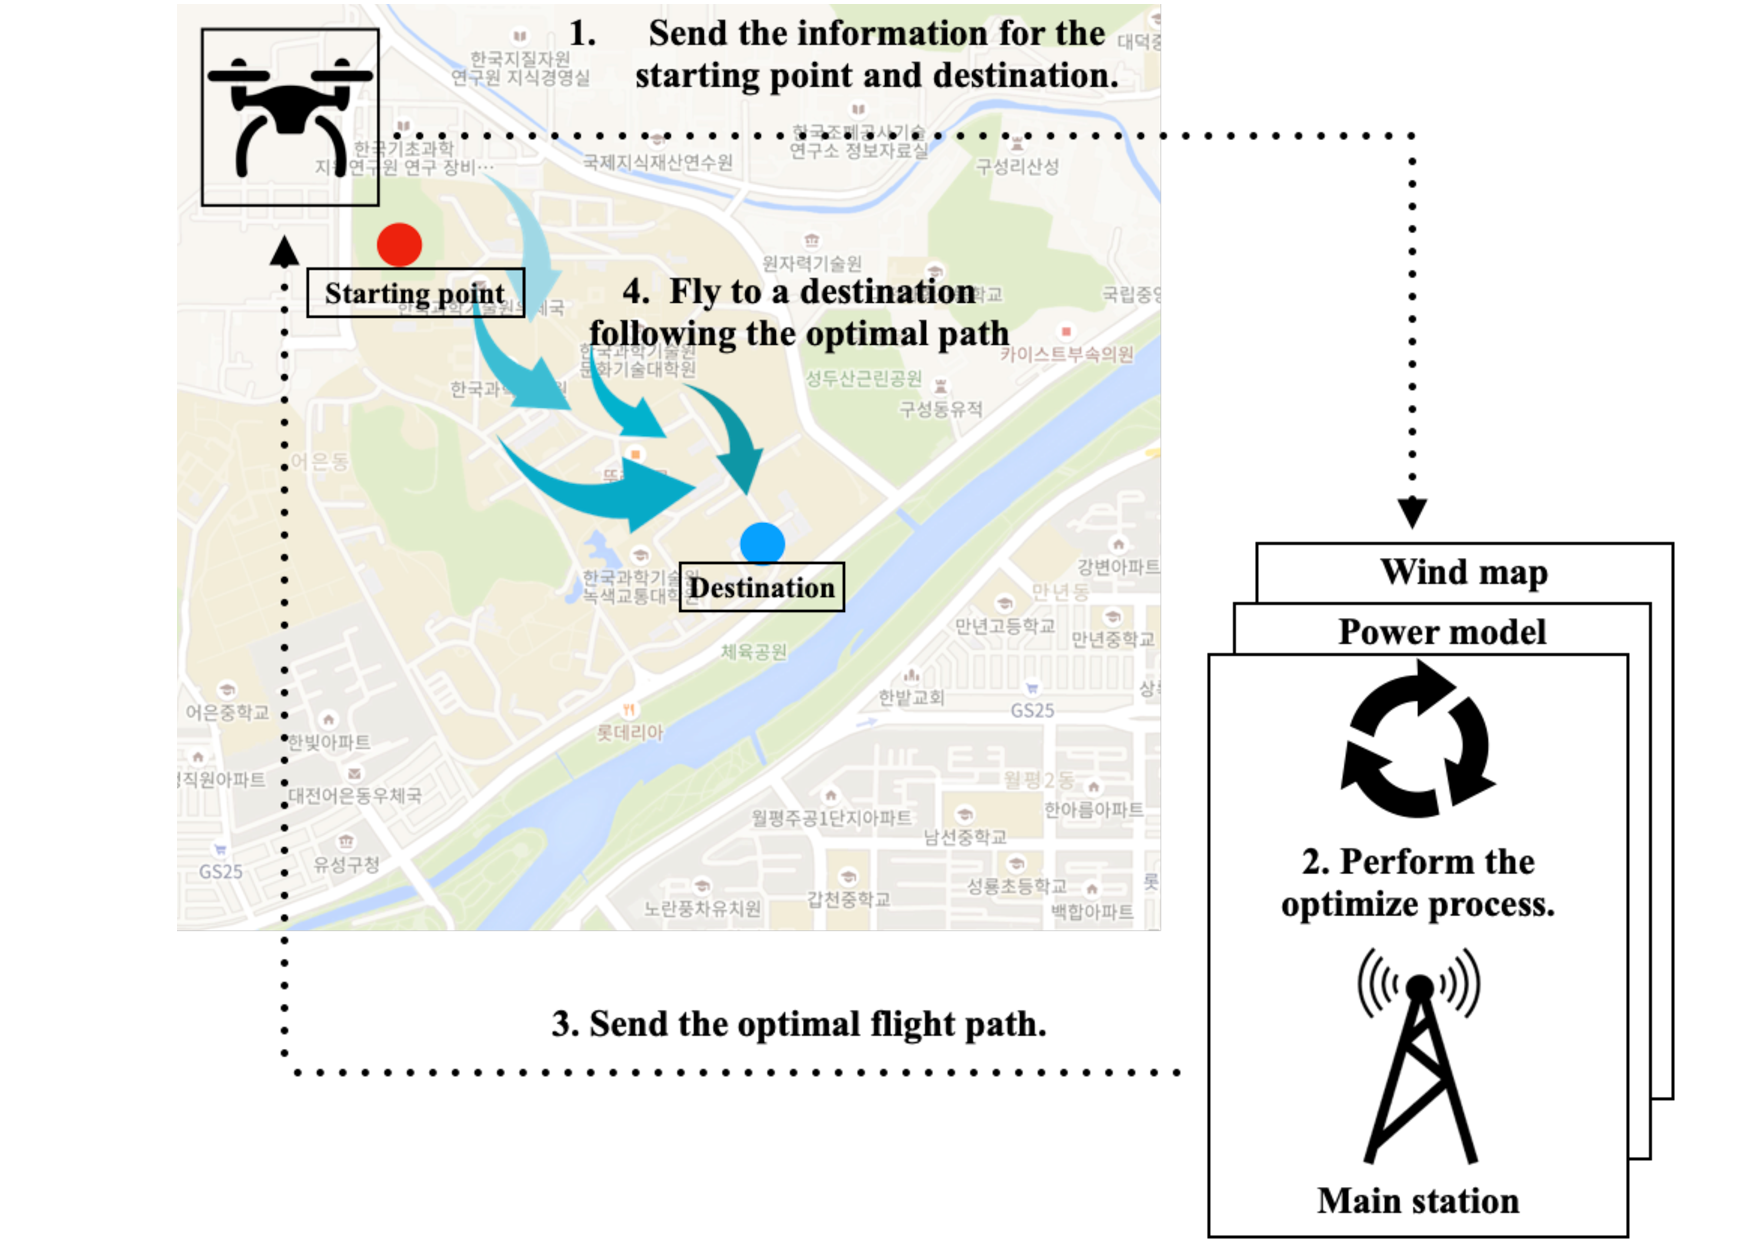
\includegraphics[scale=0.34]{fig8/problem_formulation.pdf}~\\
    \textcolor{red}{Fig. 8. The scenario of the drone optimization process.}~\\
    \justify\textcolor{red}{In our scenario, the operator inputs information about a starting point and a destination to the main station to assign a task to the drone, as shown in Fig.\,8.
    The station holds the power consumption model of the drone and wind maps about the operating environment, and the station derives the path between points entered from the operator.
    % Offline 최적화임을 여기서 언급
    Since the optimization is performed offline at the main station, it is impossible to modify the optimal path already drawn while the drone is running. Also, in this paper, we do not assume that the station considers the unexpected situations such as bird-strike or wind-sheer.
    % 외부 바람을 고려하기 위해 전용 툴을 쓴다는 것을 여기서 언급함
    However, we analyze the predictable external forces such as wind level and direction using the sophisticated analysis tool to take full advantage of the effects of external forces in creating the optimal path of the drone. 
    After that, the drone receives the optimized path from the station and then runs to the destination along the path. We formulate the flight energy optimization problem of the drone as the following:}

    \textcolor{red}{
    \vspace{7pt}
    \hrule
    \vspace{5pt}
    \noindent\textit{\textbf{Flight energy optimization problem formulation}}
    \vspace{5pt}
    \hrule
    \vspace{5pt}
    \noindent Workspace $W$ is a subset of $\mathbb{R}^3$ that drones can maneuver, and $F(\cdot)$, $B(\cdot)$ take the $W$ as the domain:\\
    \indent Workspace, \textit{$W\subset\mathbb{R}^3$, $w_n=(x_n,y_n,z_n)$, $w_n \in W$ }\\
    \indent Blockage, \textit{$BL(w_n)=bl_n$}, while blockage $bl_n\in\{0,1\}$\\
    \indent Wind field, \textit{$F(w_n) = (windx_n, windy_n)$}, while $windx_n$ is  
    x-axis wind velocity and $windy_n$ is y-axis wind velocity
    at $w_n$, respectively.
    \vspace{5pt}
    \hrule
    \vspace{5pt}
    \noindent\textit{\textbf{Given:}}~\\
    \indent $W, F(\cdot), BL(\cdot)$~\\
    \indent Set of delivery missions, $M = \{m_1, ..., m_J\},$~\\ 
    \indent $m_j = (from, to, package\;volume, package\;weight)$~\\
    \noindent\textit{\textbf{Control knob:}}~\\
    \indent Path, finite sequence of $(w,v)$,~\\
    \indent $R = \{(w_0,v_0), ..., (w_N,v_N)\}$, while $v$ is a velocity vector.
    ~\\
    \noindent\textit{\textbf{Objective:}}~\\ 
    \indent Minimize total consumption energy~\\
    \indent\indent $\sum_{j=1}^J E(m_j,R_j)$,~\\
    \indent while $E$ is energy consumption for the delivery mission $m_j$ through a path $R_j$, which satisfies~\\
    \indent\indent $BL(w_n) = 0, \forall w_n \in \bigcup_{1}^J R_j,$~\\
    \indent\indent $E(m_j, R_j) \leq$ Initial battery capacity.
    \vspace{5pt}
    \hrule
    \vspace{5pt}
    }
    \vspace{5pt}
    \textcolor{red}{In our optimization problem, the workspace $W$ where the drone is operated, the wind information $F$ in the horizontal directions provided through the discretized wind map, and the information of obstacles in the environment $BL$ are $Given$ information.
    The starting point and destination of the mission, and information of the payload are also $Given$ information.
    We define the function $Path$ using $w$ within the $W$ and the velocity of the drone $v$ as $R$, and we use the function $Path$ as our control knob.
    Our objective is to find $Path$ that minimizes the function $E$ of the energy through the optimization process when a base station receives the mission $m$ from a drone.
    The energy function $E$ cannot exceed the initial battery capacity, $BL$ must be zero for all $w$, and $Path$ consists only of $w$ presented in $W$.}
    \end{mdframed} 
    ~\\
    ~\\
	\item \textit
    {
	R6-2:  
    The Dijkstra algorithm selects a node from the queue and searches all adjacent nodes to adjust the priority. When searching all queues, select the edge with the smallest cost and infers the optimal energy path.
    In R-4, We already presented Algorithm 2 and explained the process of solving the optimization problem using the Dijkstra algorithm line-by-line.
	}
	~\\
	~\\
    \item \textbf
    {
	C7: In the VII section, the total time of each resulting path is expected to be presented.  This will help readers to evaluate the trade-off between energy and time.
	}
	\item \textit
	{
	R7: We added information about each path's traveling time in Table~IV so that readers can easily examine our optimization results.  
    In general, the energy consumption of the drone increases as it takes more time to reach the destination. However, Case 1 shows an impressive result. 
    We aimed that find a way to reduce the drone's energy consumption by optimizing the path to the influence of the external environment without significant hardware improvements, and the result shows that even if the drone flies for about 3 seconds longer than the baseline, the optimal path consumes less energy than the baseline.  
	}
    ~\\
	~\\
	\textbf{We modified Table~IV in the manuscripts as follows (Page 14.)}\\
    \begin{mdframed}[ linewidth=.75pt, userdefinedwidth=0.9\textwidth]
     \textcolor{red}{\textbf{Table IV.} Comparison of the energy consumption between the baseline and the optimal path affected by wind in each case.}  
    \centering
    \label{tab: opt.result}
    %\resizebox{\textwidth}{!}{%
    \textcolor{red}{
    \begin{tabular}{|c|c|c|c|c|c|c|}
    \hline
    \multirow{2}{*}{} & \multirow{2}{*}{Wind map} & \multicolumn{2}{c|}{Energy consumption (kJ)} & \multicolumn{2}{c|}{Travel time (sec)} & \multirow{2}{*}{Saved energy (\%)} \\ \cline{3-6}
                        &            & Baseline & Optimal path & Baseline               & Optimal path &      \\ \hline
    \multirow{2}{*}{Case 1.} & Fig.~13~(i) & 38.1     & 36.2         & \multirow{2}{*}{44.10} & 40.84        & 5.3 \\ \cline{2-4} \cline{6-7} 
                        & Fig.~13~(g) & 46.3     & 45.4         &                        & 46.53        & 1.8  \\ \hline
    \multirow{2}{*}{Case 2.} & Fig.~13~(i) & 44.7     & 43.9         & \multirow{2}{*}{53.58} & 50.68        & 1.9  \\ \cline{2-4} \cline{6-7} 
                        & Fig.~13~(h) & 45.7     & 45.4         &                        & 52.33        & 0.7  \\ \hline
    \end{tabular}%
    }
    %}
    \end{mdframed} 
    \textbf{We also modified Section~VII in the manuscripts as follows (Page 14, Line ZZ.)}\\
    \begin{mdframed}[ linewidth=.75pt, userdefinedwidth=0.9\textwidth]
    \textcolor{red}{Especially, Case 1 shows an impressive result. 
    We aim that find a way to reduce the drone's energy consumption by optimizing the path to the influence of the external environment without significant hardware improvements, and the result shows that even if the drone flies for about 3 seconds longer than the baseline, the optimal path consumes less energy than the baseline.}
    \end{mdframed}
    ~\\
	~\\
\end{description}

%\bibliographystyle{ieeetr}
%\bibliography{RR1.bib}
\end{document}